\documentclass[11pt,a4paper]{article}

\usepackage[margin=1in]{geometry}
\usepackage{amsmath,amssymb,amsthm,mathtools}
\usepackage{booktabs}
\usepackage{array}
\usepackage{microtype}
\usepackage{graphicx}
\usepackage{xcolor}
\usepackage{algorithm}
\usepackage{algpseudocode}
\usepackage[colorlinks=true,linkcolor=blue!70!black,citecolor=green!50!black,urlcolor=blue!80!black]{hyperref}

% Theorem environments
\theoremstyle{plain}
\newtheorem{theorem}{Theorem}[section]
\newtheorem{lemma}[theorem]{Lemma}
\newtheorem{proposition}[theorem]{Proposition}
\newtheorem{corollary}[theorem]{Corollary}

\theoremstyle{definition}
\newtheorem{definition}[theorem]{Definition}
\newtheorem{example}[theorem]{Example}

\theoremstyle{remark}
\newtheorem{remark}[theorem]{Remark}

% Key requirement callout box definition
\newcommand{\keyrequirement}[2]{%
  \par\vspace{0.85em}\noindent
  \begingroup
  \setlength{\fboxrule}{0.75pt}%
  \setlength{\fboxsep}{7.5pt}%
  \fcolorbox{blue!50!black}{blue!3}{%
    \begin{minipage}{\dimexpr\linewidth-2\fboxsep-2\fboxrule\relax}%
      {\bfseries\color{blue!70!black}[Key Requirement: #1]}\par\vspace{0.35em}%
      #2%
    \end{minipage}%
  }%
  \endgroup
  \par\vspace{0.85em}%
}
\title{\textbf{Monotonic Kolmogorov--Arnold Network (KAN) Transport Maps for L-SING: Theoretical Foundations and Monotonicity Proofs}}
\author{\textbf{Scientific Machine Learning \& Transport Map Research Team} \\
\textit{Repository: L-SING (\texttt{lsing\_sw})}}
\date{\today}

\begin{document}

\maketitle

\begin{abstract}
In the Localized Sparsity Identification for Non-Gaussian Distributions (L-SING) framework \cite{liaw2025learning}, undirected graphical models are discovered by estimating local conditional transport maps $S^k(x_{-k}, \cdot)$ that push forward continuous conditional distributions $\pi(x_k \mid x_{-k})$ to a standard normal reference measure $\eta_k = \mathcal{N}(0, 1)$. Existing implementations parameterize $S^k(x)$ using Unconstrained Monotonic Neural Networks (UMNNs) \cite{wehenkel2019unconstrained}, which guarantee target monotonicity $\partial_k S^k > 0$ via numerical quadrature (e.g., 50-node Clenshaw--Curtis grids), imposing heavy computational overhead and requiring higher-order automatic differentiation through the numerical integrator. In this work, we rigorously examine the replacement of UMNNs with Monotonic Kolmogorov--Arnold Networks (KANs). We systematically identify the monotonicity requirements dictated by measure transport, proving that strict target monotonicity is fully enforceable across single-layer, two-layer, and arbitrarily deep ($L$-layer) KANs, while retaining unconstrained expressivity along conditioning dimensions $x_{-k}$. Furthermore, we prove that Scale-Modulated Monotonic KANs (SM-KANs) strictly preserve target monotonicity while overcoming the inherent additive polarization dilemma of standard KANs on multiplicative non-Gaussian dependencies. We present both an intuitive, accessible explanation and formal mathematical proofs, connecting our results with the recently established MonoKAN framework \cite{polomolina2025monokan} and Fritsch--Carlson monotonicity conditions \cite{fritsch1980monotone}.
\end{abstract}

\tableofcontents
\newpage

% -----------------------------------------------------------------------------
% \section{Introduction and Problem Setting}
% -----------------------------------------------------------------------------
%
% Probabilistic graphical models represent the conditional independence relationships among a collection of continuous random variables $X = (X_1, \dots, X_d) \sim \pi$ via an undirected graph $G = (V, E)$, where $V = \{1, \dots, d\}$ and edges $(j, k) \in E$ indicate direct pairwise dependence. For Gaussian distributions, the conditional independence structure is famously encoded by the sparsity pattern of the precision (inverse covariance) matrix $\Sigma^{-1}$:
% \begin{equation}
%     \Sigma^{-1}_{jk} = 0 \iff X_j \perp X_k \mid X_{-jk}.
% \end{equation}
% However, continuous real-world phenomena (e.g., gene regulatory networks, financial markets, geophysical processes) regularly exhibit marked non-Gaussianity, asymmetry, multi-modality, and nonlinear coupling, rendering parametric Gaussian estimators such as the Graphical Lasso (GLASSO) \cite{friedman2007sparse} and semi-parametric Gaussian copula transforms (nonparanormal) \cite{liu2009nonparanormal} inadequate.
%
% To discover graphical model structure without Gaussianity assumptions, Baptista et al.\ \cite{baptista2024learning} and Morrison et al.\ \cite{morrison2017beyond} established the Sparsity Identification in Non-Gaussian Distributions (SING) framework using measure transport. SING constructs a joint lower-triangular transport map $S: \mathbb{R}^d \to \mathbb{R}^d$. While theoretically sound, estimating a global multivariate transport map requires parameterizing and storing $\mathcal{O}(d^2)$ coupling terms simultaneously, which quickly becomes computationally intractable in high dimensions.
%
% To overcome this limitation, Liaw et al.\ \cite{liaw2025learning} introduced \textbf{L-SING} (Localized Sparsity Identification for Non-Gaussian Distributions). L-SING exploits the \textit{local Markov property}:
% \begin{equation}
%     \pi(x_k \mid x_{-k}) = \pi(x_k \mid x_{\operatorname{Nb}(k)}),
% \end{equation}
% which states that a variable $X_k$ is conditionally independent of all other variables outside its neighborhood $\operatorname{Nb}(k)$ given $X_{\operatorname{Nb}(k)}$. L-SING decomposes the global estimation problem into $d$ independent, parallelizable 1D conditional transport maps $S^k: \mathbb{R}^d \to \mathbb{R}$, one for each target feature $k \in \{1, \dots, d\}$.
% -----------------------------------------------------------------------------
\section{The Measure Transport Formulation in L-SING}
% -----------------------------------------------------------------------------

\begin{remark}[Context and Scope]
\textit{Note for collaborator:} For completeness and clarity of notation, the following subsections provide a self-contained re-derivation of the L-SING conditional pullback density formula and the resulting learning loss function. 
\end{remark}

\subsection{Conditional Transport Maps}

Let $\eta_k = \mathcal{N}(0, 1)$ denote the standard univariate Gaussian reference measure with Lebesgue density,
\begin{equation}
    \eta_k(z_k) = \frac{1}{\sqrt{2\pi}} \exp\left(-\frac{1}{2} z_k^2\right).
\end{equation}
For each node $k \in \{1, \dots, d\}$, L-SING seeks a conditional transport map component $S^k(x_{-k}, \cdot): \mathbb{R} \to \mathbb{R}$, $x_k \mapsto z_k = S^k(x_{-k}, x_k)$, that pushes forward the conditional probability measure $\nu_{\pi(\cdot \mid x_{-k})}$ to the standard normal reference measure $\nu_{\eta_k}$,
\begin{equation}
    S^k(x_{-k}, \cdot)_\sharp \, \nu_{\pi(\cdot \mid x_{-k})} = \nu_{\eta_k}.
    \label{eq:pushforward_measure_statement}
\end{equation}

By definition of the pushforward measure in set-integral form, for any Borel set $B \in \mathcal{B}(\mathbb{R})$,
\begin{equation}
    \mathbb{P}\Big( Z_k \in B \;\Big|\; X_{-k} = x_{-k} \Big) = \mathbb{P}\Big( X_k \in (S^k(x_{-k}, \cdot))^{-1}(B) \;\Big|\; X_{-k} = x_{-k} \Big).
\end{equation}
Expressed as Lebesgue integrals against their respective probability densities,
\begin{equation}
    \int_B \eta_k(z_k) \, dz_k = \int_{(S^k(x_{-k}, \cdot))^{-1}(B)} \pi(x_k \mid x_{-k}) \, dx_k \quad \forall B \in \mathcal{B}(\mathbb{R}).
    \label{eq:integral_equality_fundamental}
\end{equation}

\phantomsection\label{req:key_requirement_1}
\keyrequirement{1. Target Monotonicity $\partial_k S^k > 0$}{
For the fiber map $x_k \mapsto S^k(x_{-k}, x_k)$ to be an orientation-preserving diffeomorphism on $\mathbb{R}$, its derivative along the target coordinate must be strictly positive everywhere,
\begin{equation}
    \partial_k S^k(x) \coloneqq \frac{\partial S^k(x)}{\partial x_k} > 0 \quad \forall x \in \mathbb{R}^d.
    \label{eq:target_monotonicity_requirement}
\end{equation}
This ensures that the coordinate transformation $x_k \mapsto z_k$ is one-to-one, globally invertible on $\mathbb{R}$, and has a strictly positive Jacobian $|\partial_k S^k(x)| = \partial_k S^k(x) > 0$.
}

Under this strict monotonicity condition, we apply the 1D change-of-variables substitution $z_k = S^k(x_{-k}, x_k)$ to the right-hand side of \eqref{eq:integral_equality_fundamental}. As $x_k$ traverses $(S^k(x_{-k}, \cdot))^{-1}(B)$, $z_k$ traverses $B$, with infinitesimal element $dz_k = \partial_k S^k(x_{-k}, x_k) \, dx_k$. Substituting $dx_k = \frac{1}{\partial_k S^k(x_{-k}, (S^k(x_{-k}, \cdot))^{-1}(z_k))} \, dz_k$ yields,
\begin{equation}
    \int_B \eta_k(z_k) \, dz_k = \int_B \frac{\pi\Big( (S^k(x_{-k}, \cdot))^{-1}(z_k) \;\Big|\; x_{-k} \Big)}{\partial_k S^k\Big( x_{-k}, (S^k(x_{-k}, \cdot))^{-1}(z_k) \Big)} \, dz_k.
\end{equation}
Rearranging into a single integral over $B$,
\begin{equation}
    \int_B \left( \eta_k(z_k) - \frac{\pi\Big( (S^k(x_{-k}, \cdot))^{-1}(z_k) \;\Big|\; x_{-k} \Big)}{\partial_k S^k\Big( x_{-k}, (S^k(x_{-k}, \cdot))^{-1}(z_k) \Big)} \right) dz_k = 0.
\end{equation}
Since this identity must hold for \textbf{every} Borel set $B \in \mathcal{B}(\mathbb{R})$, the integrand vanishes Lebesgue-almost everywhere,
\begin{equation}
    \eta_k(z_k) = \frac{\pi\Big( (S^k(x_{-k}, \cdot))^{-1}(z_k) \;\Big|\; x_{-k} \Big)}{\partial_k S^k\Big( x_{-k}, (S^k(x_{-k}, \cdot))^{-1}(z_k) \Big)}.
\end{equation}
Substituting $z_k = S^k(x)$ and solving for the conditional density yields the exact \textbf{conditional pullback density formula},
\begin{equation}
    \pi_{S^k}(x_k \mid x_{-k}) = \eta_k(S^k(x)) \cdot |\partial_k S^k(x)| = \frac{1}{\sqrt{2\pi}} \exp\left(-\frac{1}{2}(S^k(x))^2\right) \cdot \partial_k S^k(x).
    \label{eq:pullback_density_result}
\end{equation}
Taking the natural logarithm yields the conditional log-density of the model,
\begin{equation}
    \log \pi_{S^k}(x_k \mid x_{-k}) = -\frac{1}{2}(S^k(x))^2 + \log \partial_k S^k(x) - \frac{1}{2}\log(2\pi).
    \label{eq:cond_log_likelihood}
\end{equation}

\subsection{Connection to the Learning Objective and Functional Regularization}

The training objective in L-SING is derived directly from minimizing the Kullback--Leibler (KL) divergence between the true data distribution $\pi$ and the model's pullback distribution $\pi_{S^k}$,
\begin{align}
    D_{\mathrm{KL}}(\pi \,\|\, \pi_{S^k}) &= \mathbb{E}_{X \sim \pi}\left[ \log \pi(X_k \mid X_{-k}) - \log \pi_{S^k}(X_k \mid X_{-k}) \right] \\
    &= -\mathbb{E}_{X \sim \pi}\left[ \log \pi_{S^k}(X_k \mid X_{-k}) \right] + \mathrm{const},
\end{align}
where the constant depends only on the true data entropy and does not involve the map parameters. Substituting the conditional log-pullback formula \eqref{eq:cond_log_likelihood} into this expected negative log-likelihood directly yields,
\begin{align}
    -\mathbb{E}_{X \sim \pi}\left[ \log \pi_{S^k}(X_k \mid X_{-k}) \right] &= \mathbb{E}_{X \sim \pi}\left[ \frac{1}{2}(S^k(X))^2 - \log \partial_k S^k(X) \right] + \frac{1}{2}\log(2\pi).
\end{align}
Dropping the irrelevant additive constant $\frac{1}{2}\log(2\pi)$ and replacing the expectation with an empirical Monte Carlo average over $M$ i.i.d.\ samples $\{x^{(i)}\}_{i=1}^M \sim \pi$, we obtain the empirical negative log-likelihood. To promote sparsity, a regularization term $\Phi(S^k)$ is added, leading to the regularized loss function,
\begin{equation}
    \mathcal{L}(S^k) \coloneqq \underbrace{\frac{1}{M} \sum_{i=1}^M \left[ \frac{1}{2} (S^k(x^{(i)}))^2 - \log \partial_k S^k(x^{(i)}) \right]}_{\text{Empirical Negative Log-Pullback Likelihood } -\frac{1}{M}\sum_i \log \pi_{S^k}(x^{(i)}_k \mid x^{(i)}_{-k})} + \lambda \Phi(S^k),
    \label{eq:lsing_objective}
\end{equation}
which is minimized over the space of admissible maps, $\min_{S^k \in \mathcal{S}_k} \mathcal{L}(S^k)$, subject to the strict target monotonicity constraint $\partial_k S^k(x) > 0$ ($\pi$-a.e.). The regularization penalty $\Phi(S^k)$ is defined as,
\begin{equation}
    \Phi(S^k) \coloneqq \sum_{j=1}^d \sqrt{ \frac{1}{M} \sum_{i=1}^M \left( \frac{\partial S^k(x^{(i)})}{\partial x_j} \right)^2 }.
    \label{eq:rosasco_penalty}
\end{equation}

\subsection{The Generalized Precision Matrix}

Spantini, Bigoni, and Marzouk \cite{spantini2018inference} proved that for distributions with twice-differentiable log-densities, pairwise conditional independence is characterized by the vanishing of the mixed second derivatives of the log-density,
\begin{equation}
    X_j \perp X_k \mid X_{-jk} \iff \partial_j \partial_k \log \pi(x) = 0 \quad \forall x \in \mathbb{R}^d.
\end{equation}
Because $\partial_j \partial_k \log \pi(x) = \partial_j \partial_k \log \pi(x_k \mid x_{-k})$, the entries of the \textit{generalized precision matrix} $\Omega \in \mathbb{R}^{d \times d}$ are defined as,
\begin{equation}
    \Omega_{jk} \coloneqq \mathbb{E}\left| \partial_j \partial_k \log \pi(x_k \mid x_{-k}) \right| = \mathbb{E}\left| \partial_j \partial_k \left[ -\frac{1}{2}(S^k(x))^2 + \log \partial_k S^k(x) \right] \right|.
    \label{eq:gen_precision_def}
\end{equation}
Using $N$ independent evaluation samples, the Monte Carlo estimator is,
\begin{equation}
    \widehat{\Omega}_{jk} \coloneqq \frac{1}{N} \sum_{i=1}^N \left| \partial_j \partial_k \left[ -\frac{1}{2}(S^k(x^{(i)}))^2 + \log \partial_k S^k(x^{(i)}) \right] \right|.
\end{equation}
The matrix is symmetrized via $\widehat{\Omega}_{\text{L-SING}} = \frac{1}{2}(\widehat{\Omega} + \widehat{\Omega}^T)$, the diagonal is fixed to $\widehat{\Omega}_{kk} = 1$, and values are normalized to a maximum of $1$. Edges are determined by thresholding: $(j, k) \in E \iff |\widehat{\Omega}_{jk}| > \tau$.

\phantomsection\label{req:key_requirement_2}
\keyrequirement{2. Higher Regularity ($C^3$ Smoothness)}{
Evaluating the generalized precision entries $\Omega_{jk} = \mathbb{E}|\partial_j \partial_k \log \pi(x_k \mid x_{-k})|$ requires expanding the log-derivative integrand,
\begin{align}
    \partial_j \partial_k \left[ -\frac{1}{2}(S^k(x))^2 + \log \partial_k S^k(x) \right] &= -(\partial_j S^k)(\partial_k S^k) - S^k (\partial_j \partial_k S^k) \nonumber \\
    &\quad + \frac{(\partial_j \partial_k^2 S^k)(\partial_k S^k) - (\partial_k^2 S^k)(\partial_j \partial_k S^k)}{(\partial_k S^k)^2}.
    \label{eq:precision_integrand_expansion}
\end{align}
Consequently, the transport map $S^k$ must possess continuous derivatives up to third order ($S^k \in C^3(\mathbb{R}^d)$, or piecewise $C^3$) so that the mixed third derivative $\partial_j \partial_k^2 S^k$ is well-defined.
}

\phantomsection\label{req:key_requirement_3}
\keyrequirement{3. Efficient Derivative Computability}{
Evaluating \eqref{eq:precision_integrand_expansion} across $N$ Monte Carlo evaluation samples and all $d^2$ pairs $(j, k)$ must be computationally tractable. Under numerical quadrature architectures (such as UMNNs), this requires backpropagating three times through a numerical integrator, creating massive memory footprints and runtime bottlenecks. The transport map should ideally admit closed-form, analytic derivatives to allow direct, instantaneous precision matrix extraction.
}
% -----------------------------------------------------------------------------
\section{Limitations of Existing Architectures: MLPs and UMNNs}
% -----------------------------------------------------------------------------

\subsection{The Convexity Trap of Monotonic MLPs}

In standard Multi-Layer Perceptrons (MLPs), enforcing monotonicity with respect to an input $x_k$ requires constraining network weights along that input's computational path to be non-negative ($W \ge 0$) and using non-decreasing activation functions (e.g., ReLU or Sigmoids). However, a well-known result by Archer and Wang \cite{archer1993application} proves that constraining MLP weights to be non-negative with convex activation functions forces the entire neural network to be \textbf{globally convex} \cite{liu2020certified}. 

This creates a fundamental bottleneck for transport maps: a convex function cannot model sigmoidal transitions, S-curves, multi-modal density transformations, or higher-order inflections without introducing severe model bias (see Figure~\ref{fig:monotonic_profiles_convexity}).
\begin{figure}[htbp]
\centering
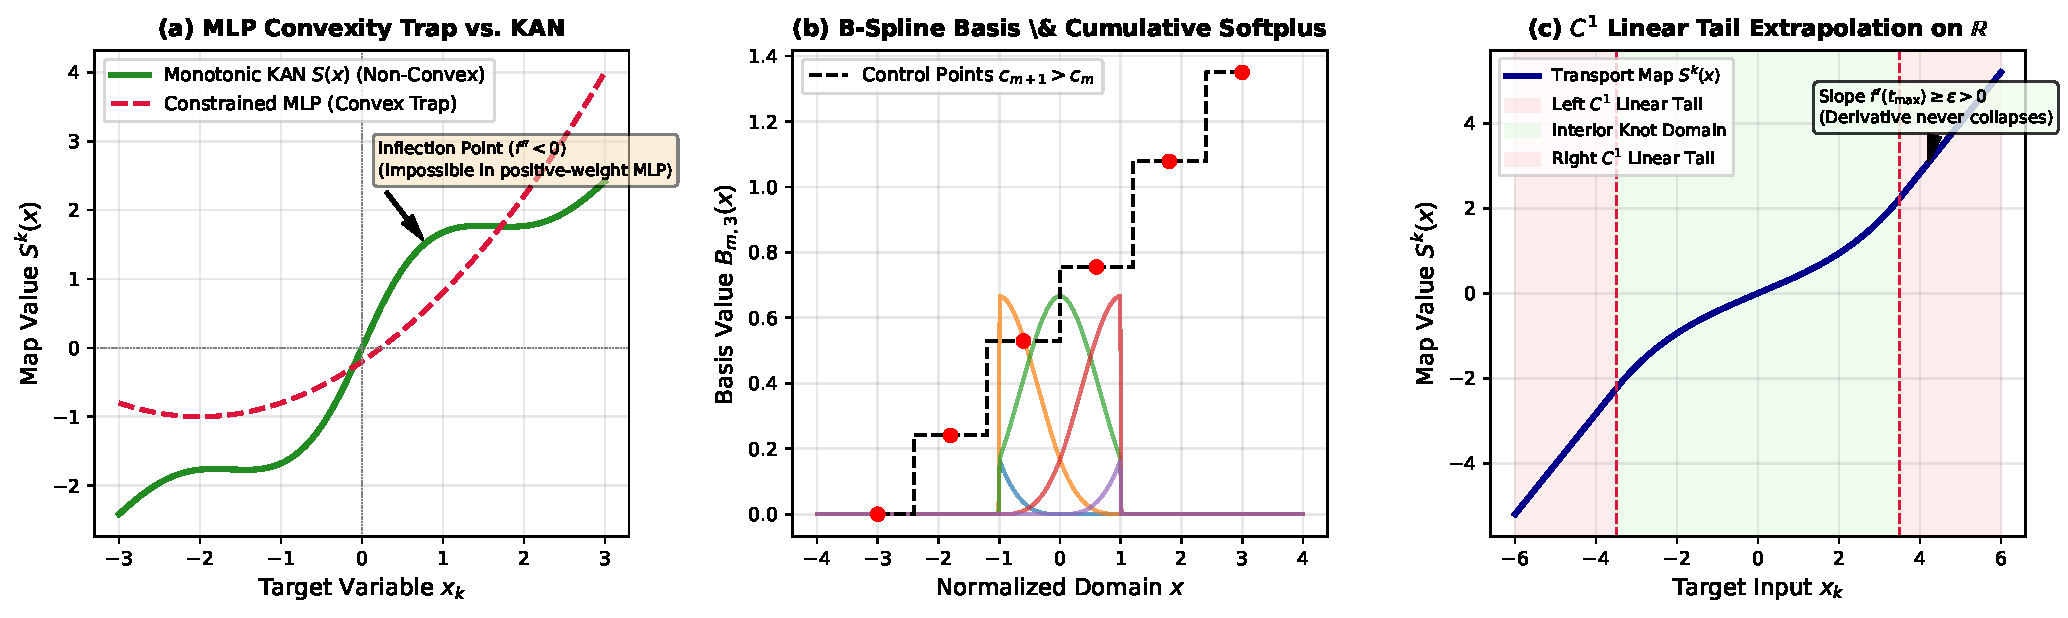
\includegraphics[width=\textwidth]{figures/fig2_monotonic_profiles_and_convexity.pdf}
\caption{\textbf{Function Expressivity and Spline Parameterization.} \textbf{(a)} The MLP convexity trap: positive-weight MLPs \cite{archer1993application} are constrained to convex curves ($f'' \ge 0$), failing to fit non-convex inflections of the target map $f(x_k)$. \textbf{(b)} Monotonic KAN representation: the learned spline $S^k(x_k)$ (green) fits the target map $f(x_k)$ (black), parameterized by strictly increasing control points $c_m$ (red dots) and the superposition of B-spline basis functions.}
\label{fig:monotonic_profiles_convexity}
\end{figure}

\subsection{The Quadrature Bottleneck of UMNNs}

To circumvent the convexity trap, the baseline L-SING implementation parameterizes $S^k(x)$ using Unconstrained Monotonic Neural Networks (UMNNs) \cite{wehenkel2019unconstrained},
\begin{equation}
    S^k(x) = \int_0^{x_k} f(t, x_{-k}; \psi) \, dt + \beta(x_{-k}),
    \label{eq:umnn_def}
\end{equation}
where $f: \mathbb{R}^d \to \mathbb{R}^+$ is an unconstrained neural network strictly constrained to positive outputs via $\exp(\cdot)$ or $\operatorname{softplus}(\cdot)$.

While UMNNs guarantee $\partial_k S^k(x) = f(x; \psi) > 0$ strictly by construction, evaluating $S^k(x)$ requires numerical integration,
\begin{equation}
    S^k(x) \approx x_k \sum_{m=1}^{N_{\text{quad}}} w_m f\left( x_k \tau_m, x_{-k}; \psi \right),
\end{equation}
typically using a 50-node Clenshaw--Curtis quadrature grid per sample. This introduces several major computational drawbacks:
\begin{enumerate}
    \item \textbf{Evaluation Overhead:} Each forward evaluation of $S^k(x)$ requires $N_{\text{quad}} = 50$ forward passes through the network $f$, increasing training and evaluation runtimes by orders of magnitude.
    \item \textbf{Nested Autodiff Through Quadrature:} Computing the Rosasco penalty $\Phi(S^k)$ requires taking first derivatives $\partial_j S^k$, requiring backpropagation through the 50-point numerical summation. Computing the generalized precision matrix entries $\widehat{\Omega}_{jk}$ requires third-order automatic differentiation through the numerical quadrature graph, leading to massive GPU/CPU memory consumption and slow extraction times (e.g., $>200$ seconds for $d=40$).
\end{enumerate}

% -----------------------------------------------------------------------------
\section{Admissibility Requirements for the Transport Map \texorpdfstring{$S^k$}{S\textasciicircum k}}
% -----------------------------------------------------------------------------

To replace the UMNN parameterization, we must formalize the exact conditions that an admissible transport map $S^k$ must fulfill.

\begin{definition}[Transport Map Admissibility Criteria]
\label{def:admissibility_criteria}
A parameterization of $S^k: \mathbb{R}^d \to \mathbb{R}$ is admissible for L-SING if and only if it satisfies the following criteria:
\begin{enumerate}
    \item \phantomsection\label{crit:target_monotonicity}\textbf{Strict Target Positivity / Invertibility (\hyperref[req:key_requirement_1]{Key Requirement~1}):}
    \begin{equation}
        \partial_k S^k(x) \coloneqq \frac{\partial S^k(x)}{\partial x_k} \ge \epsilon > 0 \quad \forall x \in \mathbb{R}^d.
    \end{equation}
    This ensures that $S^k(x_{-k}, \cdot)$ is a 1D orientation-preserving diffeomorphism on $\mathbb{R}$, guaranteeing the existence of a unique inverse pushforward and preventing numerical divergence $\log \partial_k S^k(x) \to -\infty$.
    
    \item \phantomsection\label{crit:global_domain}\textbf{Global Real-Line Domain ($\mathbb{R}^d$ Extrapolation):}
    The condition $\partial_k S^k(x) \ge \epsilon > 0$ must hold everywhere on $\mathbb{R}^d$, including outside the compact empirical training domain or spline knot interval $[t_{\min}, t_{\max}]$.
    
    \item \phantomsection\label{crit:c3_smoothness}\textbf{Higher Regularity / $C^3$ Smoothness (\hyperref[req:key_requirement_2]{Key Requirement~2}):}
    To evaluate the generalized precision integrand,
    \begin{equation}
        T_{jk}(x) = \partial_j \partial_k \left[ -\frac{1}{2}(S^k(x))^2 + \log \partial_k S^k(x) \right],
    \end{equation}
    $S^k$ must possess continuous derivatives up to order 3 ($S^k \in C^3(\mathbb{R}^d)$, or piecewise continuous 3rd derivatives), ensuring that the mixed derivative $\partial_j \partial_k^2 S^k$ is well-defined.
    
    \item \phantomsection\label{crit:conditioning_freedom}\textbf{Conditioning Freedom (Unconstrained on $x_{-k}$):}
    For all $j \neq k$, the derivative $\partial_j S^k(x)$ must be \textbf{unconstrained in sign}. The conditioning relationship must be capable of learning arbitrary, non-monotonic, multimodal responses to faithfully capture complex conditional distributions $\pi(x_k \mid x_{-k})$.
\end{enumerate}
\end{definition}

\begin{remark}[Mandatory Requirements and Desirable Properties]
\label{rem:admissibility_synthesis}
Beyond these mandatory requirements, an even further nice-to-have is \textbf{efficient derivative computability} (\hyperref[req:key_requirement_3]{Key Requirement~3}). In Section~\ref{sec:kan_theoretical_framework}, we turn to Kolmogorov--Arnold Networks (KANs), establishing a parameterization framework that not only certifies all four mandatory admissibility criteria by construction, but also natively delivers closed-form, analytic derivative evaluations.
\end{remark}

% -----------------------------------------------------------------------------
\section{Theoretical Framework and Monotonicity Proofs for KANs}
\label{sec:kan_theoretical_framework}
% -----------------------------------------------------------------------------

The architectural foundation of Kolmogorov--Arnold Networks (KANs) \cite{liu2024kan} is rooted in the Kolmogorov--Arnold representation theorem \cite{kolmogorov1957representation}, which establishes that any continuous multivariate function on a compact domain can be expressed as a finite superposition of continuous univariate functions and additions.

\begin{theorem}[Kolmogorov--Arnold Representation Theorem \cite{kolmogorov1957representation}]
\label{thm:kart}
Let $f: [0, 1]^d \to \mathbb{R}$ be an arbitrary continuous multivariate function. Then $f$ admits the exact representation,
\begin{equation}
    f(x_1, \dots, x_d) = \sum_{q=1}^{2d+1} \Phi_q \left( \sum_{p=1}^d \phi_{q, p}(x_p) \right),
    \label{eq:kart}
\end{equation}
where $\Phi_q: \mathbb{R} \to \mathbb{R}$ and $\phi_{q, p}: [0, 1] \to \mathbb{R}$ are continuous univariate functions.
\end{theorem}

While the classical theorem proves representation existence with functions that may be fractal or non-smooth, modern KANs (Liu et al.\ \cite{liu2024kan}) operationalize this principle by parameterizing the univariate edge functions with smooth, continuously differentiable splines (such as B-splines) and generalizing the structure to arbitrary network depths $L \ge 2$ and layer widths.

As illustrated in Figure~\ref{fig:kan_mlp}, KANs invert the classical MLP design: where MLPs place fixed non-linear activations $\sigma$ on nodes and learnable linear weights on edges, KANs place learnable 1D spline functions $\phi$ directly on edges and simple summations $\sum$ at nodes. Crucially, each KAN layer $l \in \{1, \dots, L\}$ with $n_{l-1}$ inputs and $n_l$ outputs forms a matrix of 1D functions,
\begin{equation}
    \mathbf{\Phi}_l = \begin{pmatrix}
        \phi_{l, 1, 1}(\cdot) & \cdots & \phi_{l, 1, n_{l-1}}(\cdot) \\
        \vdots & \ddots & \vdots \\
        \phi_{l, n_l, 1}(\cdot) & \cdots & \phi_{l, n_l, n_{l-1}}(\cdot)
    \end{pmatrix},
    \label{eq:kan_layer_matrix}
\end{equation}
updating node activations via $x^{(l)}_j = \sum_{i=1}^{n_{l-1}} \phi_{l, j, i}(x^{(l-1)}_i)$ from input $x^{(0)} = x$. A deep KAN of depth $L \ge 2$ is then simply the functional composition $\operatorname{KAN}(x) = (\mathbf{\Phi}_L \circ \cdots \circ \mathbf{\Phi}_1)(x)$, directly bridging the classical 2-layer theorem to deep expressive representations.

\begin{figure}[htbp]
\centering
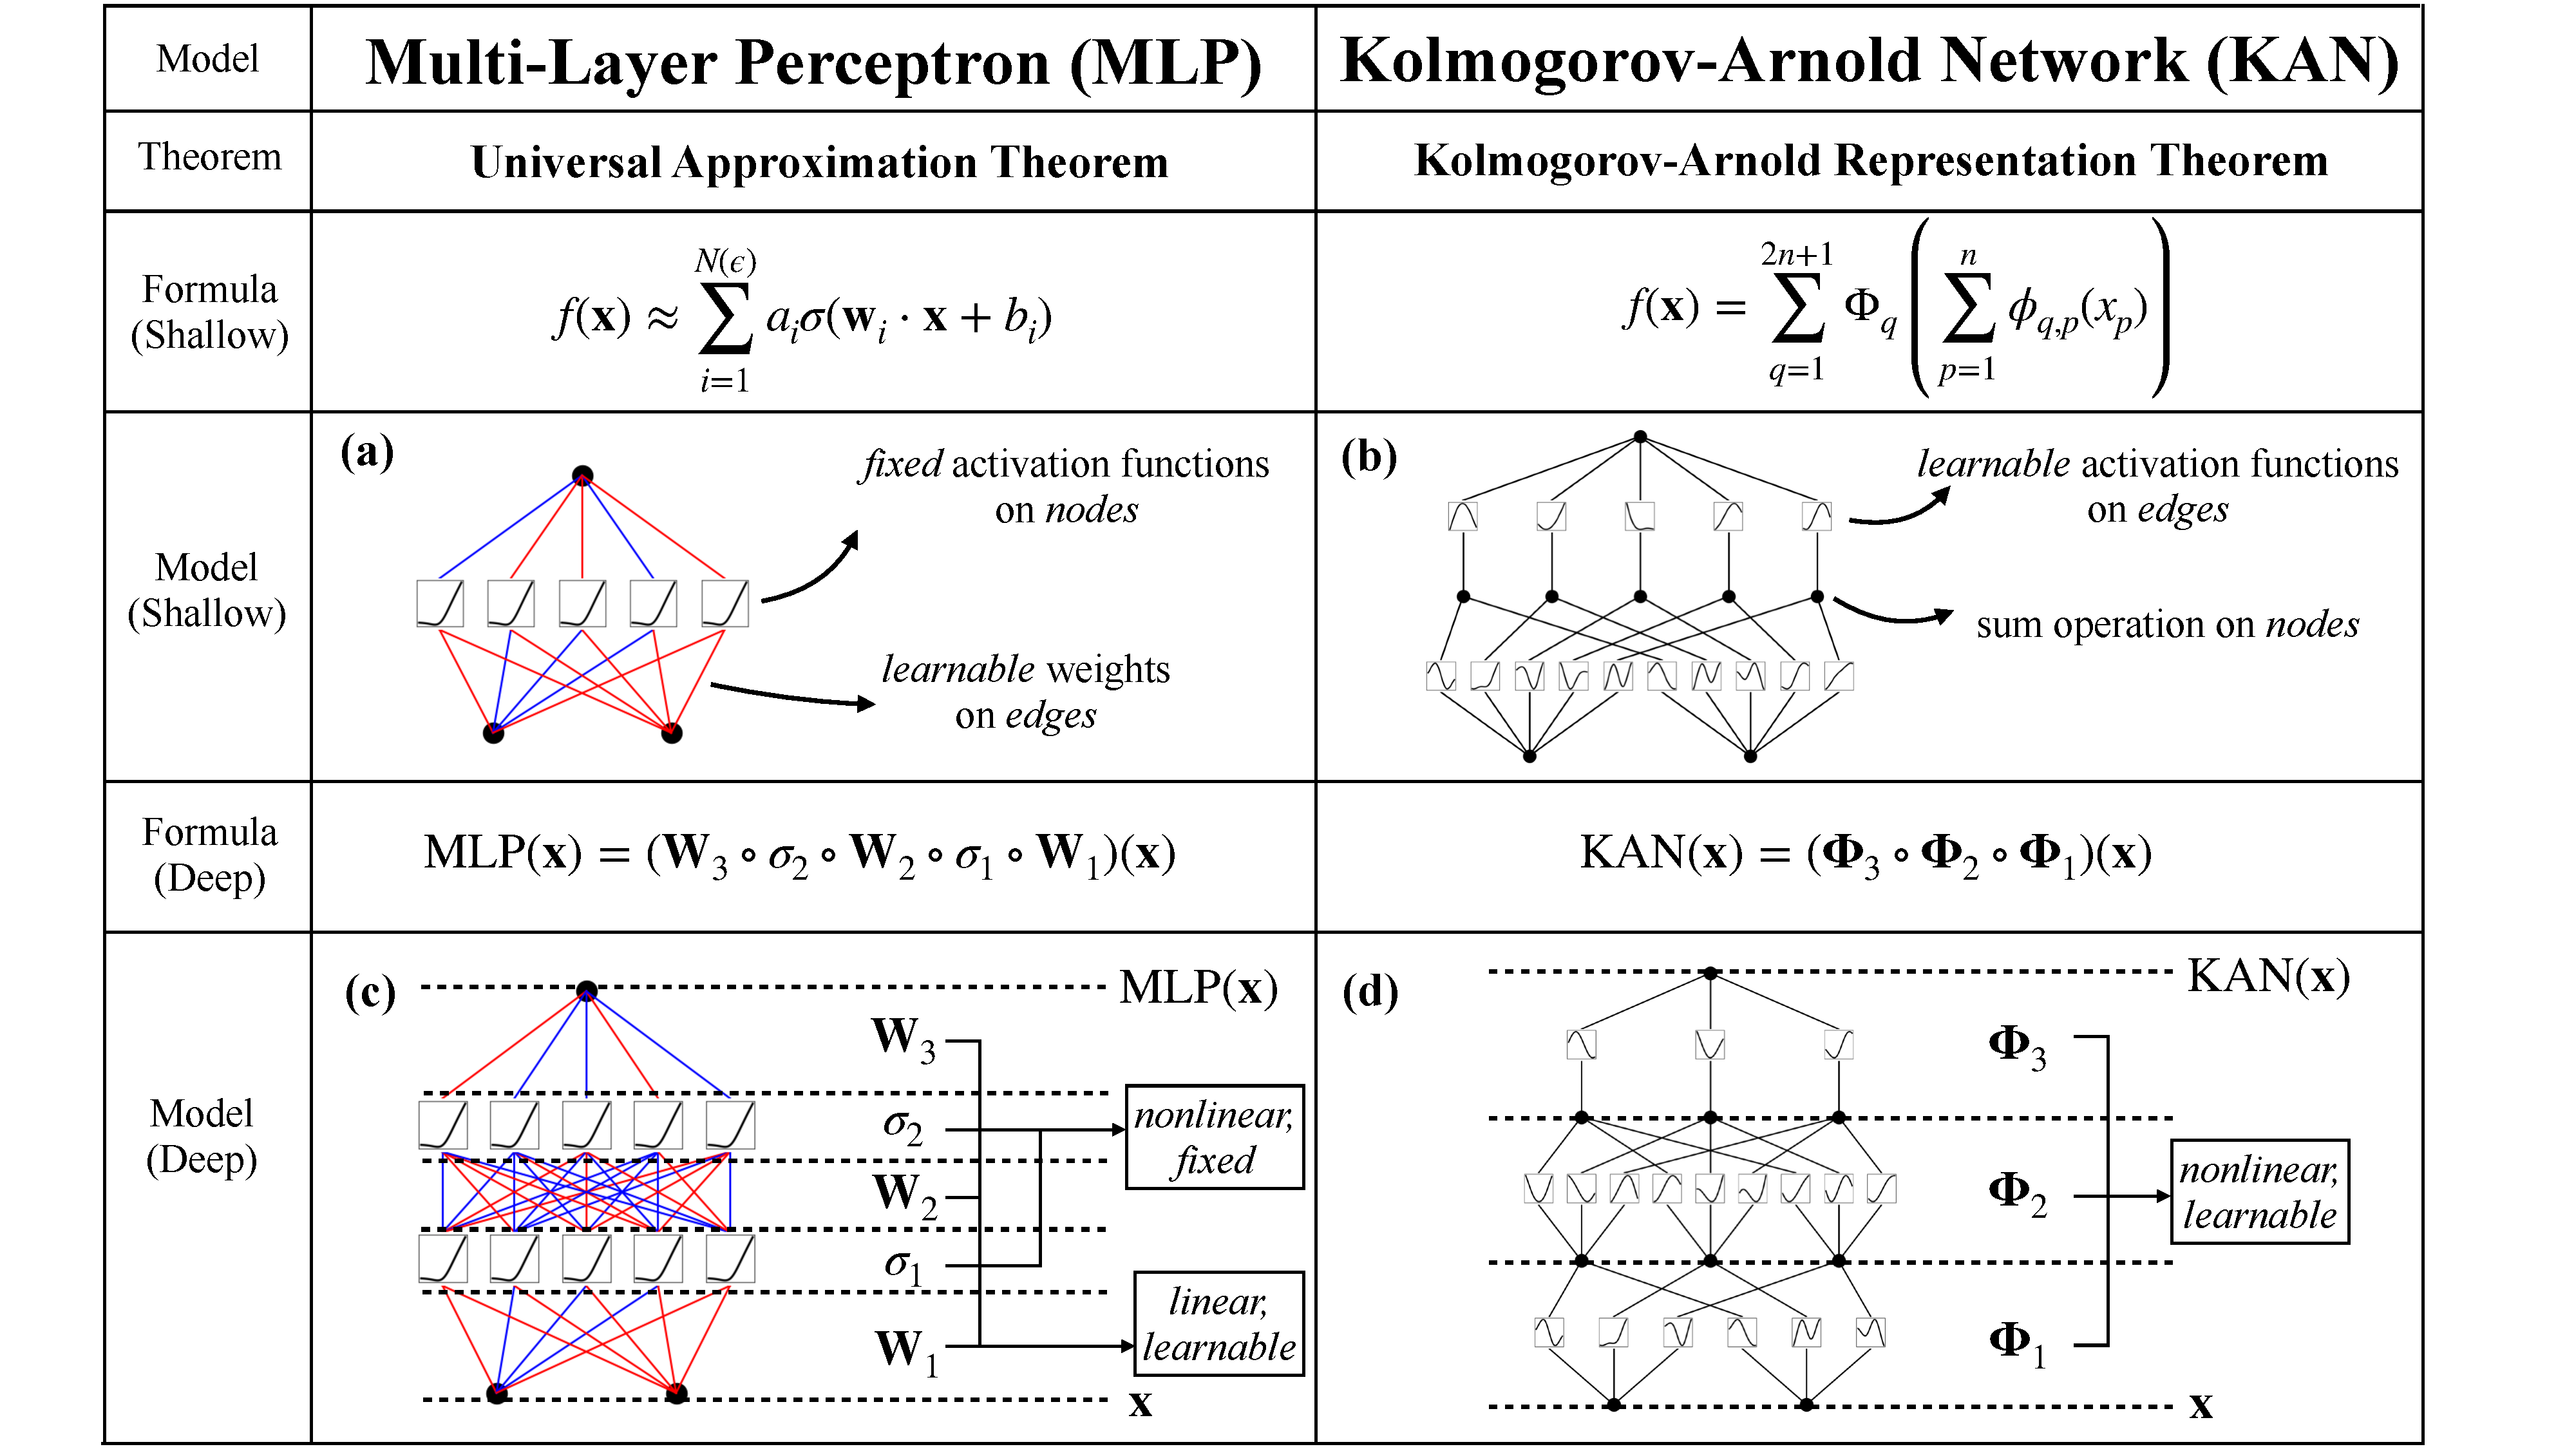
\includegraphics[width=0.92\linewidth]{figures/liu_kan_mlp.pdf}
\caption{\textbf{Architectural Comparison: Multi-Layer Perceptrons (MLPs) vs.\ Kolmogorov--Arnold Networks (KANs)} (reproduced from Liu et al.\ \cite{liu2024kan}, Figure~0.1). \textbf{(a) MLP Layer:} Fixed non-linear activation functions $\sigma(\cdot)$ (e.g., ReLU, SiLU) reside on nodes (neurons), while learnable scalar linear weights $W$ reside on edges, computing $x^{(l)} = \sigma(W_l x^{(l-1)})$. \textbf{(b) KAN Layer:} Learnable activation functions (parameterized as smooth 1D B-splines $\phi(x)$) reside directly on edges, while receiving nodes perform simple linear addition $\sum$ without non-linearities. This 2-layer graph $[d \to 2d+1 \to 1]$ provides the direct computational realization of the classical Kolmogorov--Arnold representation theorem \eqref{eq:kart}. \textbf{(c) Deep MLP Architecture:} Stacks multiple layers by interleaving affine weight matrices $W$ and static node non-linearities: $\operatorname{MLP}(x) = (W_L \circ \sigma \circ \cdots \circ W_1)x$. \textbf{(d) Deep KAN Architecture:} Generalizes the edge-activation principle to arbitrary depths $L \ge 2$ and layer widths $[n_0, n_1, \dots, n_L]$. Each layer transition $l \in \{1, \dots, L\}$ applies an $n_l \times n_{l-1}$ function matrix of 1D splines $\mathbf{\Phi}_l = (\phi_{l, j, i})$ followed by summation ($x^{(l)}_j = \sum_{i=1}^{n_{l-1}} \phi_{l, j, i}(x^{(l-1)}_i)$), defining the deep functional composition $\operatorname{KAN}(x) = (\mathbf{\Phi}_L \circ \cdots \circ \mathbf{\Phi}_1)(x)$.}
\label{fig:kan_mlp}
\end{figure}

We now establish that the admissibility requirements of Definition~\ref{def:admissibility_criteria} can be certified constructively using B-splines. We first isolate the 1D B-spline monotonicity property as a foundational lemma, demonstrate why additive ($L=1$) splines are structurally insufficient for conditional independence discovery, and then analyze the canonical two-layer ($L=2$) KAN before generalizing to arbitrary network depths.

% -----------------------------------------------------------------------------
\subsection{Foundational Lemma: Monotonic 1D B-Splines}
\label{subsec:bspline_foundation}
% -----------------------------------------------------------------------------

The fundamental mathematical building block across our monotonic KAN architectures is the univariate B-spline with ordered control points. Crucially, enforcing monotonicity at discrete control points guarantees monotonicity of the entire continuous spline curve.

\begin{lemma}[Monotonicity of 1D B-Splines]
\label{lem:bspline_mono}
Let $\phi(t) = \sum_{m=1}^M c_m B_{m, p}(t)$ be a univariate B-spline of degree $p \ge 1$ defined over a non-decreasing knot sequence $t_1 \le t_2 \le \dots \le t_{M+p+1}$ with $t_{m+p} > t_m$ for all $m \in \{2, \dots, M\}$. If the control coefficients are non-decreasing ($c_{m+1} - c_m \ge 0$), then $\phi'(t) \ge 0$ everywhere on the internal active domain $[t_{p+1}, t_{M+1}]$. Moreover, if the control coefficients satisfy strictly positive increments,
\begin{equation}
    c_{m+1} - c_m \ge \delta > 0 \quad \forall m \in \{1, \dots, M-1\},
    \label{eq:bspline_diff_condition}
\end{equation}
then $\phi'(t) \ge \epsilon > 0$ everywhere on $[t_{p+1}, t_{M+1}]$. Combined with $C^1$-continuous linear tail extrapolation, both derivative bounds ($\phi'(t) \ge 0$ and $\phi'(t) \ge \epsilon > 0$, respectively) hold globally for all $t \in \mathbb{R}$.
\end{lemma}

\begin{proof}
By the standard derivative recurrence for B-splines of degree $p$,
\begin{equation}
    \phi'(t) = p \sum_{m=2}^M \frac{c_m - c_{m-1}}{t_{m+p} - t_m} B_{m, p-1}(t).
    \label{eq:bspline_deriv_expansion}
\end{equation}
Because the basis functions of degree $p-1$ satisfy $B_{m, p-1}(t) \ge 0$ and form a partition of unity on $[t_{p+1}, t_{M+1}]$ with positive knot spans $t_{m+p} - t_m > 0$, $\phi'(t)$ is a convex combination of scaled coefficient differences. Whenever $c_m - c_{m-1} \ge 0$, every term in \eqref{eq:bspline_deriv_expansion} is non-negative, yielding $\phi'(t) \ge 0$. Under the strict increment condition $c_m - c_{m-1} \ge \delta > 0$, $\phi'(t)$ is a convex combination of strictly positive quantities,
\begin{equation}
    \phi'(t) \ge \min_m \left( \frac{p\,\delta}{t_{m+p} - t_m} \right) \coloneqq \epsilon > 0.
\end{equation}
With linear tail extrapolation maintaining constant boundary slopes ($\phi'(t) = \phi'(t_{\text{boundary}})$) outside the active knot interval (Section~\ref{subsec:linear_extrapolation}), non-negativity and strict positivity extend over the entire real line $\mathbb{R}$.
\end{proof}

\begin{remark}[Why Additive Splines ($L=1$) Cannot Discover General Graph Structure]
\label{rem:single_layer_failure}
Consider a purely additive single-layer spline transport map $S^k(x) = \phi_k(x_k) + \sum_{j \neq k} \phi_j(x_j)$. Applying Lemma~\ref{lem:bspline_mono} to $\phi_k$ immediately guarantees $\partial_k S^k(x) = \phi'_k(x_k) \ge \epsilon > 0$.

However, because the conditioning coordinates enter purely additively, the target derivative $\partial_k S^k(x) = \phi'_k(x_k)$ is completely independent of $x_{-k}$, so all mixed cross-derivatives of the map vanish identically,
\begin{equation}
    \partial_j \partial_k S^k(x) = \frac{\partial}{\partial x_j} [\phi'_k(x_k)] \equiv 0 \quad \text{and} \quad \partial_j \partial_k \log \partial_k S^k(x) \equiv 0 \quad \forall j \neq k.
\end{equation}
In the generalized precision expansion \eqref{eq:precision_integrand_expansion}, both the interaction term $-S^k(\partial_j \partial_k S^k)$ and the log-Jacobian coupling term vanish, reducing the integrand to the separable rank-one product $-(\partial_j S^k)(\partial_k S^k) = -\phi'_j(x_j)\phi'_k(x_k)$. Geometrically, $x_{-k}$ can only induce a rigid location shift without modulating conditional scale, variance, or higher-order shape; for any zero-mean scale or shape coupling, $\phi_j \equiv 0$ and $\Omega_{jk}$ in \eqref{eq:gen_precision_def} collapses to zero. Functional composition ($L \ge 2$) is therefore mathematically necessary to achieve $\partial_j \partial_k S^k(x) \not\equiv 0$.
\end{remark}

% -----------------------------------------------------------------------------
\subsection{Two-Layer Monotonic KAN as the Primary Workhorse}
\label{subsec:two_layer_kan}
% -----------------------------------------------------------------------------

Having established that additive splines fail the graphical model recovery requirement, we focus on the canonical two-layer KAN $[d \to Q \to 1]$ illustrated in Figure~\ref{fig:2layer_kan_liu}. This architecture directly operationalizes the classical Kolmogorov--Arnold representation theorem (Theorem~\ref{thm:kart}) and serves as the primary parameterization for local transport maps $S^k$.

\begin{definition}[Two-Layer Monotonic KAN]
\label{def:kan_2layer}
A 2-layer KAN transport map $S^k: \mathbb{R}^d \to \mathbb{R}$ ($L=2$) with $n_1 = Q$ hidden summation nodes and input $x^{(0)} = x$ is parameterized via,
\begin{equation}
    S^k(x) = x^{(2)}_1 = \sum_{q=1}^Q \phi_{2, 1, q}\big( x^{(1)}_q(x) \big),
    \label{eq:kan_2layer}
\end{equation}
where $x^{(1)}_q(x)$ denotes the $q$-th hidden activation at layer $l=1$,
\begin{equation}
    x^{(1)}_q(x) \coloneqq \phi_{1, q, k}(x_k) + \sum_{j \neq k} \phi_{1, q, j}(x_j),
    \label{eq:hidden_activation_uq}
\end{equation}
and the edge activations satisfy:
\begin{enumerate}
    \item \textbf{Target Inner Splines ($l=1$):} $\phi_{1, q, k}: \mathbb{R} \to \mathbb{R}$ are non-decreasing univariate B-splines ($\phi'_{1, q, k} \ge 0$), parameterized via Lemma~\ref{lem:bspline_mono}.
    \item \textbf{Outer Splines ($l=2$):} $\phi_{2, 1, q}: \mathbb{R} \to \mathbb{R}$ are non-decreasing univariate B-splines ($\phi'_{2, 1, q} \ge 0$), with at least one active path $q^* \in \{1, \dots, Q\}$ satisfying $\phi'_{1, q^*, k} \ge \epsilon_1 > 0$ and $\phi'_{2, 1, q^*} \ge \epsilon_2 > 0$, parameterized via Lemma~\ref{lem:bspline_mono}.
    \item \textbf{Conditioning Inner Splines ($l=1$):} $\phi_{1, q, j}: \mathbb{R} \to \mathbb{R}$ ($j \neq k$) are arbitrary unconstrained univariate B-splines.
\end{enumerate}
\end{definition}

\begin{figure}[!htbp]
\centering
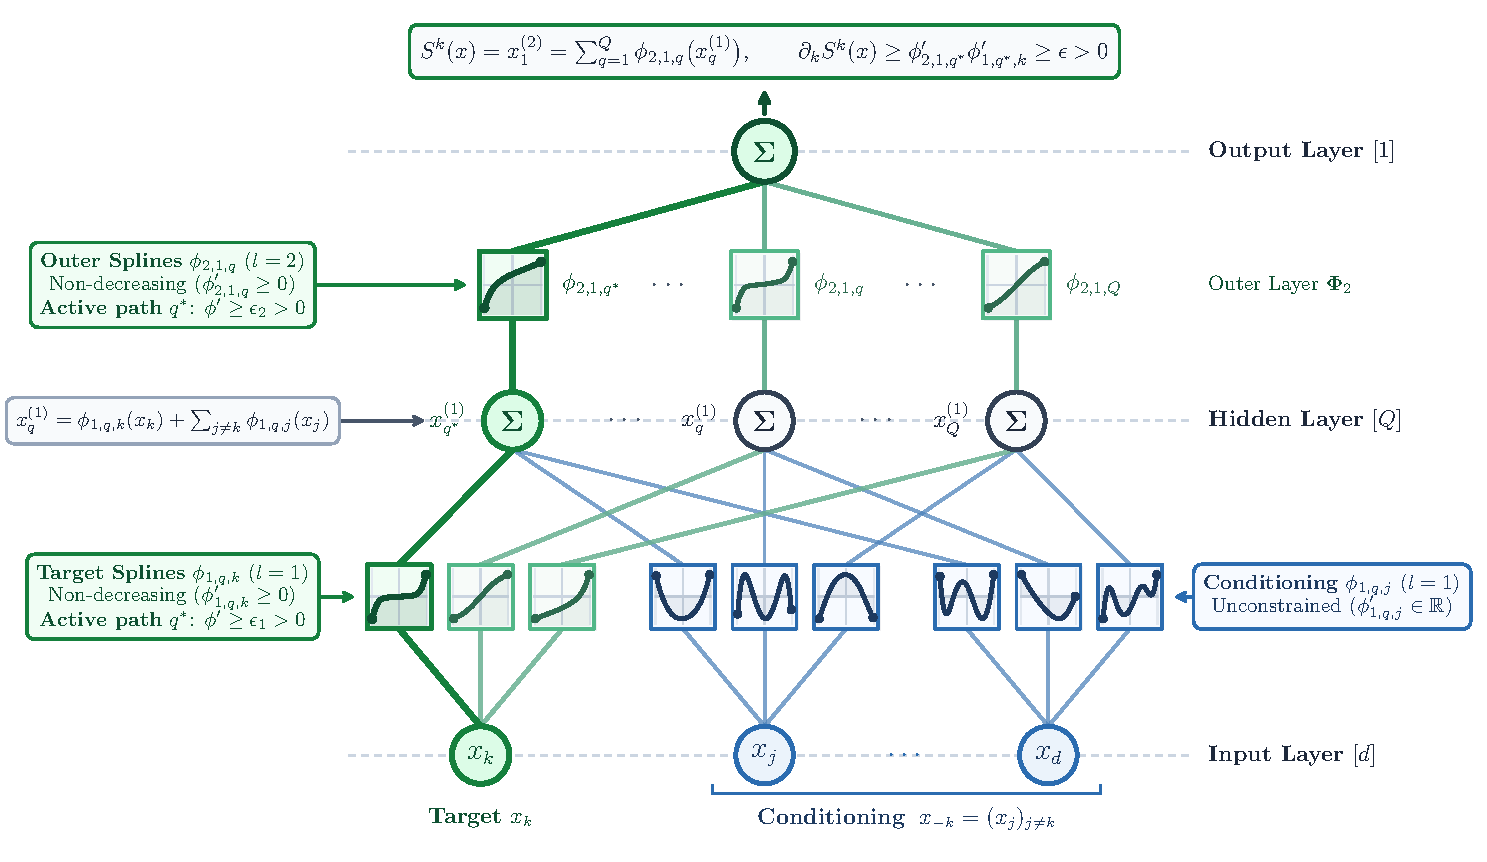
\includegraphics[width=\textwidth]{figures/fig_2layer_kan_liu.pdf}
\caption{\textbf{Two-Layer Monotonic KAN Transport Map $S^k: \mathbb{R}^d \to \mathbb{R}$ with Topology $[d \to Q \to 1]$} (following the edge-activation diagram convention of Liu et al.~\cite{liu2024kan}). Input coordinates $x^{(0)} = x$ partition into the target feature $x_k$ (green) and conditioning features $x_{-k} = (x_j)_{j \neq k}$ (blue), while hidden nodes $x^{(1)}_q$ and the output node $x^{(2)}_1 = S^k(x)$ perform linear summations ($\sum$). Each edge carries a learnable 1D B-spline plot: target inner splines $\phi_{1,q,k}(x_k)$ and outer splines $\phi_{2,1,q}(x^{(1)}_q)$ are non-decreasing ($\phi'_{1,q,k} \ge 0$, $\phi'_{2,1,q} \ge 0$, muted green), and the certified active path through hidden node $x^{(1)}_{q^*}$ (highlighted in bold dark green) maintains strictly positive derivatives $\phi'_{1,q^*,k} \ge \epsilon_1 > 0$ and $\phi'_{2,1,q^*} \ge \epsilon_2 > 0$, guaranteeing $\partial_k S^k(x) \ge \epsilon_1 \epsilon_2 > 0$ globally on $\mathbb{R}^d$, whereas conditioning inner splines $\phi_{1,q,j}(x_j)$ remain unconstrained (blue).}
\label{fig:2layer_kan_liu}
\end{figure}

\begin{theorem}[Admissibility and Structural Coupling in 2-Layer KANs]
\label{thm:2layer_kan_admissibility}
Let $S^k$ be parameterized according to Definition~\ref{def:kan_2layer}. Then,
\begin{enumerate}
    \item \textbf{Target Monotonicity (\hyperref[crit:target_monotonicity]{Criterion~1}):} For all $x \in \mathbb{R}^d$, the target derivative satisfies,
    \begin{equation}
        \partial_k S^k(x) = \sum_{q=1}^Q \phi'_{2, 1, q}\big(x^{(1)}_q(x)\big) \cdot \phi'_{1, q, k}(x_k) \ge \epsilon > 0,
        \label{eq:2layer_target_monotonicity}
    \end{equation}
    where $\epsilon \coloneqq \epsilon_1 \epsilon_2 > 0$ is a uniform positive constant, certifying that $S^k(x_{-k}, \cdot)$ is a 1D orientation-preserving diffeomorphism on $\mathbb{R}$.
    
    \item \textbf{Conditioning Freedom and Structural Coupling (\hyperref[crit:conditioning_freedom]{Criterion~4}):} For any conditioning coordinate $j \neq k$, the conditioning splines $\phi_{1, q, j}$ are unconstrained in sign, and the mixed second derivative is given analytically by,
    \begin{equation}
        \partial_j \partial_k S^k(x) = \sum_{q=1}^Q \phi''_{2, 1, q}\big(x^{(1)}_q(x)\big) \cdot \phi'_{1, q, j}(x_j) \cdot \phi'_{1, q, k}(x_k).
        \label{eq:2layer_mixed_deriv}
    \end{equation}
    Consequently, $\partial_j \partial_k S^k(x) \not\equiv 0$ in general whenever the outer splines exhibit non-zero curvature, allowing unconstrained modeling of conditional dependencies and full recovery of the generalized precision matrix $\Omega$.
\end{enumerate}
\end{theorem}

\begin{proof}
Differentiating $S^k(x)$ in \eqref{eq:kan_2layer} with respect to $x_k$ via the multivariable chain rule yields,
\begin{equation}
    \partial_k S^k(x) = \sum_{q=1}^Q \frac{\partial \phi_{2, 1, q}(x^{(1)}_q)}{\partial x^{(1)}_q} \cdot \frac{\partial x^{(1)}_q(x)}{\partial x_k} = \sum_{q=1}^Q \phi'_{2, 1, q}\big(x^{(1)}_q(x)\big) \cdot \phi'_{1, q, k}(x_k).
\end{equation}
By Lemma~\ref{lem:bspline_mono}, all target inner and outer splines satisfy $\phi'_{1, q, k} \ge 0$ and $\phi'_{2, 1, q} \ge 0$ globally on $\mathbb{R}$, ensuring every product term in the sum is non-negative. For the designated active path $q^*$, the product satisfies $\phi'_{2, 1, q^*}(x^{(1)}_{q^*}(x)) \cdot \phi'_{1, q^*, k}(x_k) \ge \epsilon_1 \epsilon_2 \eqqcolon \epsilon > 0$. Decomposing the summation into the active path $q^*$ and the remaining non-negative paths yields $\partial_k S^k(x) \ge \epsilon + 0 = \epsilon > 0$ for all $x \in \mathbb{R}^d$.

Next, differentiating $\partial_k S^k(x)$ with respect to conditioning variable $x_j$ ($j \neq k$) via the chain rule pulls out the inner derivative $\partial_j x^{(1)}_q(x) = \phi'_{1, q, j}(x_j)$, yielding \eqref{eq:2layer_mixed_deriv}. Because $\phi_{1, q, j}$ is unconstrained, $\phi'_{1, q, j}(x_j)$ can take arbitrary real values, and the second derivative of the outer spline $\phi''_{2, 1, q}(x^{(1)}_q(x))$ is likewise unconstrained in sign while maintaining $\phi'_{2, 1, q} \ge 0$. Thus, $\partial_j \partial_k S^k(x)$ is generally non-zero, allowing the map to capture non-Gaussian dependency structures.
\end{proof}

\begin{remark}[Remaining Criteria: Domain Extrapolation, Regularity, and Analytic Differentiation]
\label{rem:remaining_criteria_synthesis}
The remaining criteria of Definition~\ref{def:admissibility_criteria} follow naturally from the spline construction:
\textbf{Global Extrapolation (\hyperref[crit:global_domain]{Criterion~2})} is satisfied by attaching $C^1$ linear tails outside the knot domain (Section~\ref{subsec:linear_extrapolation});
\textbf{$C^3$ Smoothness (\hyperref[crit:c3_smoothness]{Criterion~3})} is satisfied by selecting B-spline degree $p = 3$ for piecewise continuous third derivatives ($C^2$ across interior knots) or $p \ge 4$ for continuous third derivatives on the interior knot domain; and
\textbf{Derivative Computability (\hyperref[req:key_requirement_3]{Key Requirement~3})} is fulfilled natively because all derivatives in \eqref{eq:2layer_target_monotonicity} and \eqref{eq:2layer_mixed_deriv} are available in closed form via standard B-spline recurrence, bypassing the nested numerical quadrature required by UMNNs.
\end{remark}
% -----------------------------------------------------------------------------
\subsection{Arbitrarily Deep Multi-Layer KAN (\texorpdfstring{$L$}{L} Layers)}

We now generalize the construction to a KAN of arbitrary depth $L \ge 2$, with layer dimensions $[n_0, n_1, n_2, \dots, n_L]$, where $n_0 = d$ (input features) and $n_L = 1$ (scalar output $S^k(x)$), as illustrated in Figure~\ref{fig:deep_kan_liu}.

\begin{definition}[Arbitrarily Deep Monotonic KAN]
\label{def:deep_mono_kan}
\label{def:deep_kan}
Let $S^k: \mathbb{R}^d \to \mathbb{R}$ be an $L$-layer KAN ($L \ge 2$) with layer dimensions $[n_0, n_1, \dots, n_L]$, where $n_0 = d$ (input features) and $n_L = 1$ (scalar transport map output). Setting the input layer to $x^{(0)} = x \in \mathbb{R}^d$, the network computes intermediate activations layer-by-layer for $l \in \{1, \dots, L\}$,
\begin{equation}
    x^{(l)}_j = \sum_{i=1}^{n_{l-1}} \phi_{l, j, i}\big(x^{(l-1)}_i\big), \quad j = 1, \dots, n_l,
    \label{eq:kan_layer_def}
\end{equation}
where $\phi_{l, j, i}: \mathbb{R} \to \mathbb{R}$ is the learnable univariate B-spline on the edge from neuron $i$ in layer $l-1$ to neuron $j$ in layer $l$. The full transport map $S^k(x) \coloneqq x^{(L)}_1$ represents the $L$-fold functional composition,
\begin{equation}
    S^k(x) = \Big( \mathbf{\Phi}_L \circ \mathbf{\Phi}_{L-1} \circ \cdots \circ \mathbf{\Phi}_1 \Big)(x).
    \label{eq:kan_composition_def}
\end{equation}
Let $\mathbb{P}_k$ denote the set of all directed computational paths $\mathcal{P} = (i_0, i_1, \dots, i_L)$ from target input $i_0 = k$ to output $i_L = 1$, where $i_l \in \{1, \dots, n_l\}$. The network is an \emph{admissible monotonic KAN} if its edge splines, parameterized via Lemma~\ref{lem:bspline_mono}, satisfy:
\begin{enumerate}
    \item \textbf{Target-Transmitting Splines:} Every edge emanating from target input $x_k$ at layer $l=1$ and all downstream edges across hidden and output layers ($2 \le l \le L$) are non-decreasing,
    \begin{equation}
        \phi'_{1, j, k}(t) \ge 0 \quad (\forall j \in \{1, \dots, n_1\}), \quad \text{and} \quad \phi'_{l, j, i}(t) \ge 0 \quad (\forall 2 \le l \le L, \, \forall j, i), \quad \forall t \in \mathbb{R},
    \end{equation}
    and there exists at least one active backbone path $\mathcal{P}^* = (i_0^*, i_1^*, \dots, i_L^*) \in \mathbb{P}_k$ (with $i_0^* = k$ and $i_L^* = 1$) whose edges are strictly increasing,
    \begin{equation}
        \phi'_{l, i_l^*, i_{l-1}^*}(t) \ge \epsilon_l > 0 \quad \forall t \in \mathbb{R}, \quad \forall l \in \{1, \dots, L\}.
    \end{equation}
    \item \textbf{Conditioning Splines:} For all conditioning inputs $i \neq k$ at layer $l=1$, the splines $\phi_{1, j, i}$ are unconstrained in sign, derivative, and magnitude.
\end{enumerate}
\end{definition}

\begin{figure}[!htbp]
\centering
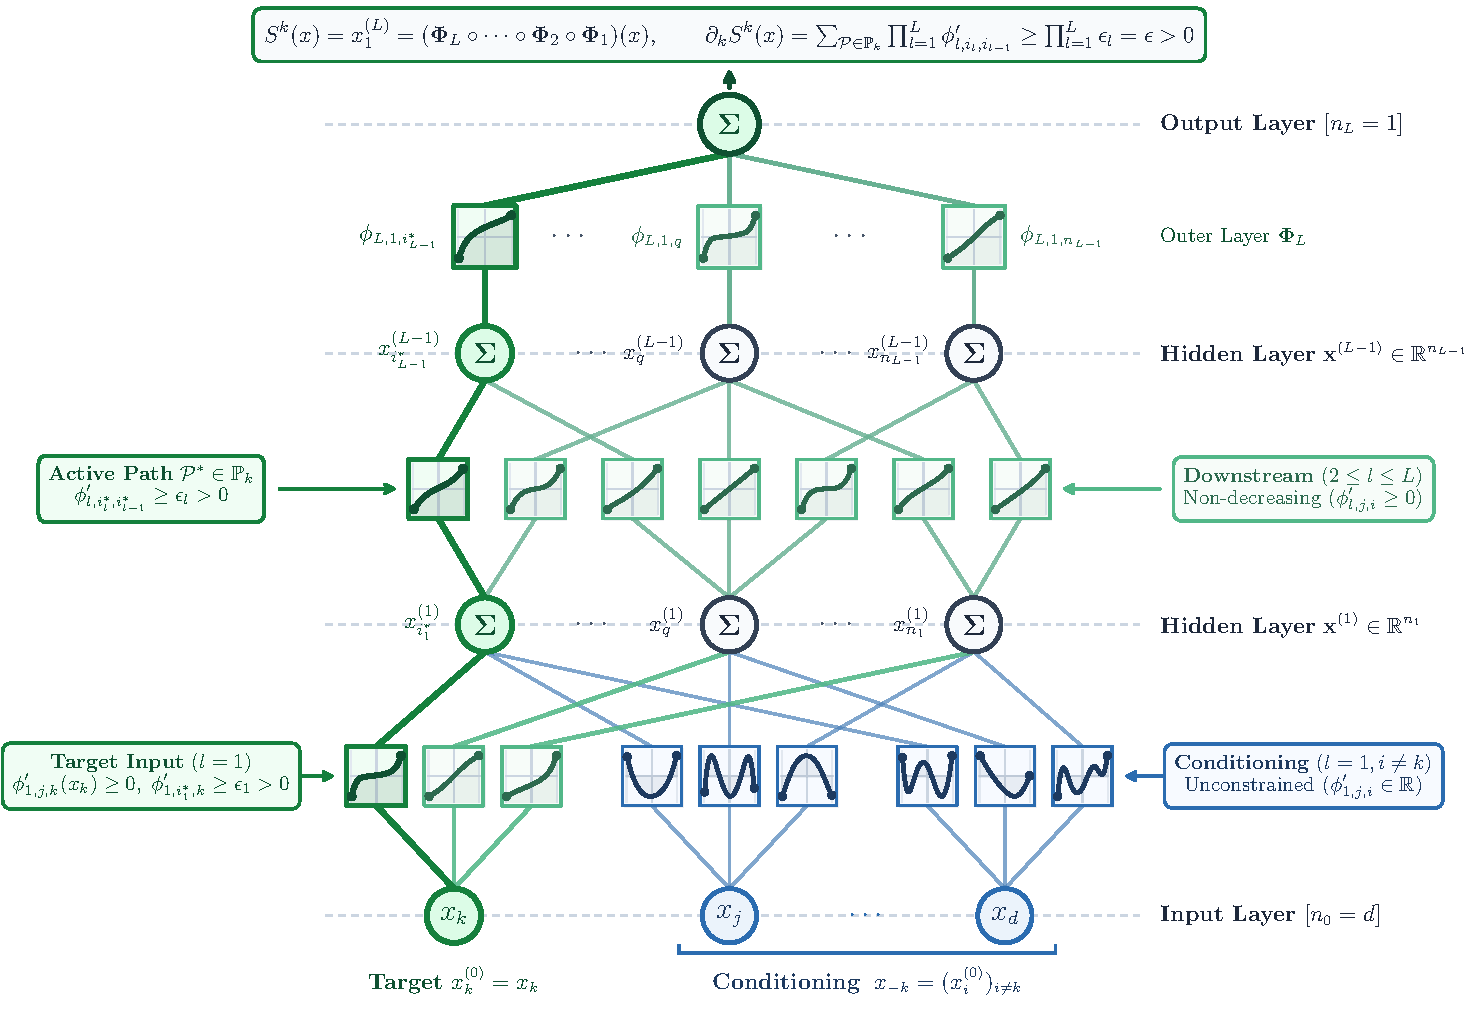
\includegraphics[width=\textwidth]{figures/fig_deep_kan_liu.pdf}
\caption{\textbf{Arbitrarily Deep $L$-Layer Monotonic KAN Transport Map $[n_0 \to n_1 \to \cdots \to n_{L-1} \to n_L]$} ($n_0 = d, n_L = 1$; following Liu et al.~\cite{liu2024kan}, Figure~0.1d). Target edges emanating from $x_k$ at layer $l=1$ and all downstream hidden edges ($2 \le l \le L$) are non-decreasing ($\phi'_{l,j,i} \ge 0$, muted green), while conditioning edges $\phi_{1,j,i}(x_i)$ ($i \neq k$) are unconstrained (blue). At least one certified active backbone path $\mathcal{P}^* = (i_0^*, i^*_1, \dots, i^*_{L-1}, i_L^*) \in \mathbb{P}_k$ with $i_0^* = k, i_L^* = 1$ (highlighted in bold dark green) maintains strictly positive derivatives $\phi'_{l, i^*_l, i^*_{l-1}} \ge \epsilon_l > 0$, guaranteeing $\partial_k S^k(x) \ge \prod_{l=1}^L \epsilon_l = \epsilon > 0$ globally on $\mathbb{R}^d$.}
\label{fig:deep_kan_liu}
\end{figure}

\begin{theorem}[Admissibility and Certified Monotonicity for Arbitrarily Deep KANs]
\label{thm:deep_kan_mono}
Let $S^k$ be parameterized according to Definition~\ref{def:deep_mono_kan}. Then,
\begin{enumerate}
    \item \textbf{Target Monotonicity (\hyperref[crit:target_monotonicity]{Criterion~1}):} For all $x \in \mathbb{R}^d$, the target derivative satisfies,
    \begin{equation}
        \partial_k S^k(x) = \sum_{\mathcal{P} \in \mathbb{P}_k} \prod_{l=1}^L \phi'_{l, i_l, i_{l-1}}\big(x^{(l-1)}_{i_{l-1}}\big) \ge \epsilon > 0,
        \label{eq:deep_kan_target_monotonicity}
    \end{equation}
    where $\epsilon \coloneqq \prod_{l=1}^L \epsilon_l > 0$ is a uniform positive constant, certifying that $S^k(x_{-k}, \cdot)$ is a 1D orientation-preserving diffeomorphism on $\mathbb{R}$.

    \item \textbf{Conditioning Freedom (\hyperref[crit:conditioning_freedom]{Criterion~4}):} For all conditioning coordinates $i \neq k$, the conditioning splines $\phi_{1, j, i}$ are unconstrained in sign, derivative, and magnitude, allowing unrestricted nonlinear contextual modulation while strictly preserving target monotonicity.
\end{enumerate}
\end{theorem}

\begin{proof}
We evaluate the sensitivity of the transport map output $S^k(x) = x^{(L)}_1$ with respect to the target input $x_k = x^{(0)}_k$. Applying the multivariable chain rule layer by layer from the output layer $L$ back to the input layer $0$ expands the total derivative into a multi-index sum,
\begin{equation}
    \frac{\partial S^k(x)}{\partial x_k} = \frac{\partial x^{(L)}_1}{\partial x^{(0)}_k} = \sum_{i_{L-1}=1}^{n_{L-1}} \sum_{i_{L-2}=1}^{n_{L-2}} \cdots \sum_{i_1=1}^{n_1} \left( \frac{\partial x^{(L)}_1}{\partial x^{(L-1)}_{i_{L-1}}} \frac{\partial x^{(L-1)}_{i_{L-1}}}{\partial x^{(L-2)}_{i_{L-2}}} \cdots \frac{\partial x^{(1)}_{i_1}}{\partial x^{(0)}_k} \right).
    \label{eq:chain_rule_expansion}
\end{equation}
From the layer definition \eqref{eq:kan_layer_def}, intermediate neuron activations are linear superpositions of univariate edge splines, $x^{(l)}_j = \sum_{i=1}^{n_{l-1}} \phi_{l, j, i}(x^{(l-1)}_i)$. Differentiating $x^{(l)}_j$ with respect to upstream activation $x^{(l-1)}_i$, all other terms vanish, yielding the univariate spline derivative,
\begin{equation}
    \frac{\partial x^{(l)}_j}{\partial x^{(l-1)}_i} = \phi'_{l, j, i}\big(x^{(l-1)}_i\big).
\end{equation}
At the first layer $l=1$, holding all conditioning coordinates $x_{-k} = \{x_i : i \neq k\}$ fixed gives $\partial x^{(1)}_{i_1} / \partial x^{(0)}_k = \phi'_{1, i_1, k}(x^{(0)}_k)$.

Substituting these edge derivatives into \eqref{eq:chain_rule_expansion}, each term in the summation corresponds to the product of edge derivatives along a directed computational path $\mathcal{P} = (i_0, i_1, \dots, i_L) \in \mathbb{P}_k$ with $i_0 = k$ and $i_L = 1$,
\begin{equation}
    \partial_k S^k(x) = \sum_{\mathcal{P} \in \mathbb{P}_k} \prod_{l=1}^L \phi'_{l, i_l, i_{l-1}}\big(x^{(l-1)}_{i_{l-1}}\big).
    \label{eq:path_sum}
\end{equation}
By Lemma~\ref{lem:bspline_mono} and Condition~1 of Definition~\ref{def:deep_mono_kan}, all target-transmitting splines satisfy $\phi'_{l, j, i}(t) \ge 0$ globally on $\mathbb{R}$, so every path product in \eqref{eq:path_sum} is non-negative regardless of intermediate activations $x^{(l-1)}$. Isolating the certified active backbone path $\mathcal{P}^* = (i_0^*, i_1^*, \dots, i_L^*)$, along which $\phi'_{l, i_l^*, i_{l-1}^*}(t) \ge \epsilon_l > 0$, we decompose the sum as,
\begin{equation}
    \partial_k S^k(x) = \prod_{l=1}^L \phi'_{l, i_l^*, i_{l-1}^*}\big(x^{(l-1)}_{i_{l-1}^*}\big) + \sum_{\mathcal{P} \neq \mathcal{P}^*} \prod_{l=1}^L \phi'_{l, i_l, i_{l-1}}\big(x^{(l-1)}_{i_{l-1}}\big) \ge \prod_{l=1}^L \epsilon_l + 0 = \epsilon > 0.
\end{equation}
Because this strictly positive bound holds independently of intermediate activations $x^{(l-1)}$ and does not depend on $x$, $S^k(x)$ is certified strictly monotonic across all of $\mathbb{R}^d$, establishing Criterion~1.

Finally, conditioning coordinates $x_{-k}$ enter only through conditioning splines $\phi_{1, j, i}$ ($i \neq k$) at layer $l=1$. Because these splines are completely unconstrained (Condition~2 of Definition~\ref{def:deep_mono_kan}), they provide unrestricted non-linear modulation of intermediate activations without altering the non-negativity of downstream derivatives, establishing Criterion~4.
\end{proof}
% -----------------------------------------------------------------------------
\subsection{Scale-Modulated Monotonic KAN (SM-KAN)}

\subsubsection{The Additive Polarization Dilemma}
In non-Gaussian graphical models, conditional dependencies are frequently \emph{multiplicative} or \emph{scale-dependent} (heteroscedastic). Consider, for example, the benchmark Butterfly distribution,
\begin{equation}
    X_1 \sim \mathcal{N}(0, 1), \quad W \sim \mathcal{N}(0, 1), \quad X_1 \perp W, \quad X_2 = W \cdot X_1.
    \label{eq:butterfly_def}
\end{equation}
Conditioned on $X_1 = x_1 \neq 0$, the target variable follows $X_2 \mid (X_1 = x_1) \sim \mathcal{N}(0, x_1^2)$, so the exact Knothe--Rosenblatt transport map normalizing $X_2$ to a standard Gaussian is,
\begin{equation}
    S^2(x_1, x_2) = \frac{x_2}{|x_1|}, \quad x_1 \neq 0.
    \label{eq:butterfly_ideal_map}
\end{equation}
In a purely additive 2-layer KAN \eqref{eq:kan_2layer}, each hidden node combines the target spline $u_q = \phi_{1, q, k}(x_k)$ and the conditioning sum $v_q = \sum_{j \neq k} \phi_{1, q, j}(x_j)$ solely by addition, $x^{(1)}_q(x) = u_q + v_q$. Representing a multiplicative interaction $u \cdot v$ through univariate outer functions applied to sums $u \pm v$ requires algebraic polarization,
\begin{equation}
    u \cdot v = \frac{1}{4}(u + v)^2 - \frac{1}{4}(u - v)^2.
    \label{eq:polarization_identity}
\end{equation}
When we expand $(u + v)^2 = u^2 + 2uv + v^2$, isolating the cross-product $u \cdot v$ requires subtracting a second branch $-\frac{1}{4}(u - v)^2$ to cancel the unwanted marginal squares $u^2$ and $v^2$. In a standard unconstrained KAN, this subtraction is achieved by assigning negative outer spline derivatives ($\phi'_{2, 1, q} < 0$) to the second branch. Under Definition~\ref{def:kan_2layer}, however, global target monotonicity requires $\phi'_{2, 1, q}(t) \ge 0$ across all outer splines to guarantee $\partial_k S^k(x) > 0$ (and furthermore, the quadratic outer functions $t \mapsto \pm \frac{1}{4}t^2$ themselves are not monotonic on $\mathbb{R}$ since their derivatives $\pm \frac{1}{2}t$ change sign at $t = 0$). Consequently, purely additive monotonic KANs cannot represent multiplicative conditioning without violating the non-negative outer-slope constraints required for target monotonicity.

\subsubsection{Scale-Modulation Architecture}
The polarization conflict in \eqref{eq:polarization_identity} arises only when a purely additive network is forced to synthesize multiplication indirectly by squaring and subtracting sums $u \pm v$. To resolve this conflict directly, we introduce an explicit multiplicative conditioning pathway outside the core monotonic KAN: we multiply a certified monotonic core network $S^k_{\text{core}}(x)$ by a strictly positive conditioning scale factor $E(\sigma(x_{-k}))$ and add a conditioning location shift $\alpha(x_{-k})$.

Here $\sigma(x_{-k}) = \sum_{j \neq k} \psi_j(x_j)$ and $\alpha(x_{-k}) = \sum_{j \neq k} \rho_j(x_j)$ are unconstrained additive B-spline networks over the conditioning variables $x_{-k}$ (which may also be generalized to multi-layer KANs). Because $\sigma(x_{-k})$ and $\alpha(x_{-k})$ depend only on the conditioning coordinates $x_{-k}$, the product $E(\sigma(x_{-k})) \cdot S^k_{\text{core}}(x)$ is formed directly at the output without adding $x_k$ and $x_{-k}$ inside a quadratic outer spline. Consequently, no unwanted marginal squares $u^2$ or $v^2$ are generated, and no negative outer spline slopes ($\phi'_{2, 1, q} < 0$) are required to cancel them.

To ensure that the scale multiplier remains strictly positive and uniformly bounded away from zero and infinity across all of $\mathbb{R}^{d-1}$ without numerical overflow or derivative collapse in the far tails, the scalar output $\sigma(x_{-k}) \in \mathbb{R}$ is mapped to the positive scale factor through the smooth saturated exponential activation,
\begin{equation}
    E(\sigma) \coloneqq \exp\left( s_{\max} \tanh\left( \frac{\sigma}{s_{\max}} \right) \right) \in \big(e^{-s_{\max}}, e^{s_{\max}}\big),
    \label{eq:sm_kan_scale_activation}
\end{equation}
where $s_{\max} > 0$ is a fixed scale ceiling (in our implementation, $s_{\max} = 4.0$). Near the origin ($\sigma \approx 0$), $s_{\max}\tanh(\sigma / s_{\max}) \approx \sigma$, so \eqref{eq:sm_kan_scale_activation} reproduces the standard exponential scale factor $\exp(\sigma)$, while globally guaranteeing $e^{-s_{\max}} < E(\sigma) < e^{s_{\max}}$ and preserving $C^\infty$ smoothness everywhere on $\mathbb{R}$.

Placing the additive offset $\alpha(x_{-k})$ outside the product---directly analogous to the conditioning intercept $+\beta(x_{-k})$ added after the monotone integral in the UMNN parameterization \eqref{eq:umnn_def}---completes a full location--scale conditioning wrapper around $S^k_{\text{core}}(x)$. Whereas any conditioning shift inside $S^k_{\text{core}}(x)$ is multiplied by $E(\sigma(x_{-k}))$, the external offset $\alpha(x_{-k})$ shifts the standardized output $z_k = S^k(x)$ directly in the $\mathcal{N}(0, 1)$ reference space without being attenuated or amplified by the scale factor. For a general heteroscedastic Butterfly distribution with conditional mean shift $\mu(X_1)$, where $X_2 \mid (X_1 = x_1) \sim \mathcal{N}(\mu(x_1), x_1^2)$, writing the exact transport map as,
\begin{equation}
    S^2(x_1, x_2) = \frac{x_2 - \mu(x_1)}{|x_1|} = \exp\big(-\log|x_1|\big) \cdot x_2 - \frac{\mu(x_1)}{|x_1|}, \quad x_1 \neq 0,
    \label{eq:butterfly_sm_decomp}
\end{equation}
allows the core monotonic network to learn the linear identity $S^2_{\text{core}}(x_1, x_2) = x_2$ ($\partial_2 S^2_{\text{core}} = 1 > 0$), while $\sigma(x_1) = \psi_1(x_1)$ approximates $-\log|x_1|$ and $\alpha(x_1) = \rho_1(x_1)$ captures the location shift $-\mu(x_1)/|x_1|$ (recovering the centered Butterfly map \eqref{eq:butterfly_ideal_map} when $\mu(x_1) \equiv 0$; see Appendix~\ref{app:sm_kan_location_scale} for a detailed derivation).

\begin{definition}[Scale-Modulated Monotonic KAN]
\label{def:sm_kan}
A \textbf{Scale-Modulated Monotonic KAN (SM-KAN)} parameterizes the $k$-th conditional transport map $S^k: \mathbb{R}^d \to \mathbb{R}$ as,
\begin{equation}
    S^k(x) = \exp\left( s_{\max} \tanh\left( \frac{\sigma(x_{-k})}{s_{\max}} \right) \right) \cdot S^k_{\text{core}}(x) + \alpha(x_{-k}),
    \label{eq:sm_kan_def}
\end{equation}
where $s_{\max} > 0$ is a fixed scale ceiling, and:
\begin{enumerate}
    \item \textbf{Certified Monotonic Core ($S^k_{\text{core}}$):} $S^k_{\text{core}}: \mathbb{R}^d \to \mathbb{R}$ is an $L$-layer certified monotonic KAN ($L \ge 2$, parameterized according to Definition~\ref{def:kan_2layer} or Definition~\ref{def:deep_mono_kan}) satisfying $\partial_k S^k_{\text{core}}(x) \ge \epsilon > 0$ for all $x \in \mathbb{R}^d$.
    \item \textbf{Conditioning Scale Network ($\sigma$):} $\sigma: \mathbb{R}^{d-1} \to \mathbb{R}$ is an unconstrained additive B-spline network over the conditioning coordinates $x_{-k}$,
    \begin{equation}
        \sigma(x_{-k}) = \sum_{j \neq k} \psi_j(x_j),
        \label{eq:sm_kan_sigma}
    \end{equation}
    where each $\psi_j: \mathbb{R} \to \mathbb{R}$ ($j \neq k$) is an unconstrained univariate B-spline.
    \item \textbf{Conditioning Offset Network ($\alpha$):} $\alpha: \mathbb{R}^{d-1} \to \mathbb{R}$ is an unconstrained additive B-spline network over the conditioning coordinates $x_{-k}$,
    \begin{equation}
        \alpha(x_{-k}) = \sum_{j \neq k} \rho_j(x_j),
        \label{eq:sm_kan_alpha}
    \end{equation}
    where each $\rho_j: \mathbb{R} \to \mathbb{R}$ ($j \neq k$) is an unconstrained univariate B-spline.
\end{enumerate}
\end{definition}

\begin{figure}[H]
\centering
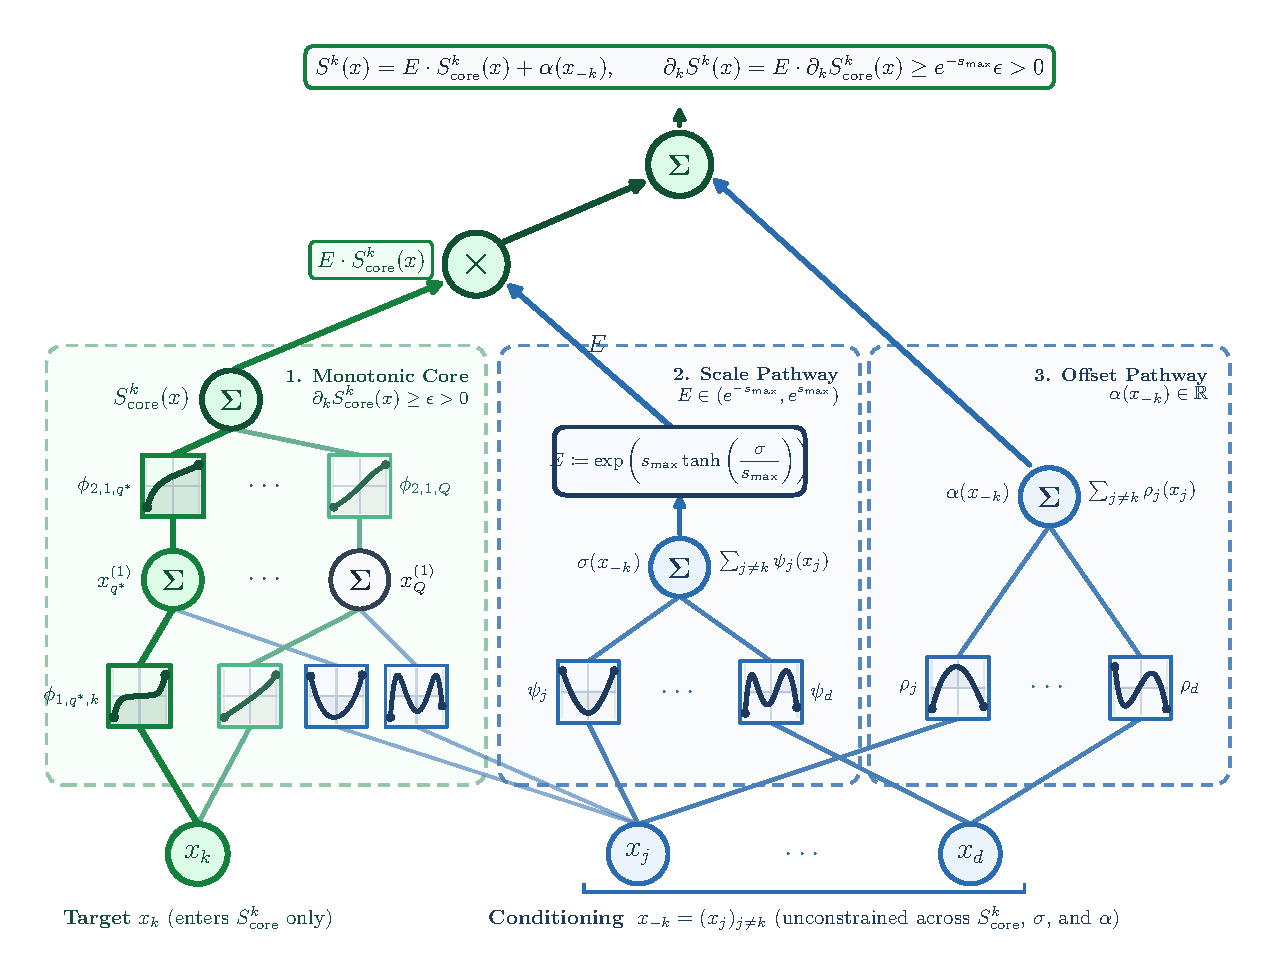
\includegraphics[width=\textwidth]{figures/fig_sm_kan_liu.pdf}
\caption{\textbf{Scale-Modulated Monotonic KAN (SM-KAN) Transport Map Architecture} (Definition~\ref{def:sm_kan}). The target coordinate $x_k$ (green) enters exclusively through the certified monotonic core network $S^k_{\text{core}}(x)$ (Module~1, left), where non-decreasing target-transmitting splines and an active path $q^*$ guarantee $\partial_k S^k_{\text{core}}(x) \ge \epsilon > 0$. Conditioning coordinates $x_{-k} = (x_j)_{j \neq k}$ (blue) modulate the map through three unconstrained pathways: internal conditioning splines within $S^k_{\text{core}}(x)$, an additive scale network $\sigma(x_{-k}) = \sum_{j \neq k} \psi_j(x_j)$ mapped through smooth saturation and exponentiation $E \coloneqq \exp(s_{\max}\tanh(\sigma/s_{\max})) \in (e^{-s_{\max}}, e^{s_{\max}})$ to a multiplication gate ($\times$) computing $E \cdot S^k_{\text{core}}(x)$ (Module~2, center), and an additive offset network $\alpha(x_{-k}) = \sum_{j \neq k} \rho_j(x_j)$ summed at the output node ($\sum$) (Module~3, right).}
\label{fig:sm_kan_liu}
\end{figure}

\begin{proposition}[Admissibility and Monotonicity Invariance Under Scale Modulation]
\label{prop:scale_modulated_mono}
Let $S^k$ be parameterized according to Definition~\ref{def:sm_kan}, and let $E(u) \coloneqq \exp(s_{\max}\tanh(u / s_{\max}))$. Then,
\begin{enumerate}
    \item \textbf{Uniform Target Monotonicity (\hyperref[crit:target_monotonicity]{Criterion~1}):} For all $x \in \mathbb{R}^d$, the target derivative satisfies,
    \begin{equation}
        \partial_k S^k(x) = E\big(\sigma(x_{-k})\big) \cdot \partial_k S^k_{\text{core}}(x) \ge e^{-s_{\max}} \cdot \epsilon \eqqcolon \epsilon_{\text{SM}} > 0,
        \label{eq:sm_derivative}
    \end{equation}
    certifying that for every fixed $x_{-k} \in \mathbb{R}^{d-1}$, the fiber map $S^k(x_{-k}, \cdot)$ is a 1D orientation-preserving diffeomorphism on $\mathbb{R}$ with uniform positive derivative lower bound $\epsilon_{\text{SM}} > 0$.
    \item \textbf{Conditioning Freedom and Multiplicative Coupling (\hyperref[crit:conditioning_freedom]{Criterion~4}):} For any conditioning coordinate $j \neq k$, the scale and offset splines $\psi_j, \rho_j$ are unconstrained in sign, and the mixed second derivative is given by,
    \begin{equation}
        \partial_j \partial_k S^k(x) = E\big(\sigma(x_{-k})\big) \left[ \operatorname{sech}^2\left(\frac{\sigma(x_{-k})}{s_{\max}}\right) \psi'_j(x_j) \cdot \partial_k S^k_{\text{core}}(x) + \partial_j \partial_k S^k_{\text{core}}(x) \right].
        \label{eq:sm_mixed_deriv}
    \end{equation}
    In particular, $\partial_j \partial_k S^k(x)$ is non-zero whenever $\psi'_j(x_j) \neq 0$, enabling unrestricted multiplicative conditioning without violating target monotonicity.
\end{enumerate}
\end{proposition}

\begin{proof}
Because $\sigma(x_{-k})$ and $\alpha(x_{-k})$ depend only on conditioning coordinates $x_{-k}$, they are constant with respect to target coordinate $x_k$, so $\partial_k [E(\sigma(x_{-k}))] \equiv 0$ and $\partial_k \alpha(x_{-k}) \equiv 0$. Differentiating \eqref{eq:sm_kan_def} with respect to $x_k$ yields,
\begin{equation}
    \partial_k S^k(x) = E\big(\sigma(x_{-k})\big) \cdot \partial_k S^k_{\text{core}}(x).
\end{equation}
Since $\tanh(u) > -1$ for all $u \in \mathbb{R}$, we have $E(\sigma(x_{-k})) > e^{-s_{\max}}$. Combined with $\partial_k S^k_{\text{core}}(x) \ge \epsilon > 0$ from Condition~1 of Definition~\ref{def:sm_kan}, this yields the uniform bound $\partial_k S^k(x) \ge e^{-s_{\max}} \epsilon \eqqcolon \epsilon_{\text{SM}} > 0$ across all $x \in \mathbb{R}^d$, establishing Criterion~1.

Differentiating $\partial_k S^k(x)$ with respect to conditioning coordinate $x_j$ ($j \neq k$) via the product rule gives $\partial_j \partial_k S^k(x) = \partial_j [E(\sigma(x_{-k}))] \cdot \partial_k S^k_{\text{core}}(x) + E(\sigma(x_{-k})) \cdot \partial_j \partial_k S^k_{\text{core}}(x)$. Applying the chain rule to $E(\sigma(x_{-k}))$,
\begin{equation}
    \partial_j \big[ E(\sigma(x_{-k})) \big] = E\big(\sigma(x_{-k})\big) \cdot \operatorname{sech}^2\left(\frac{\sigma(x_{-k})}{s_{\max}}\right) \cdot \partial_j \sigma(x_{-k}).
\end{equation}
Substituting $\partial_j \sigma(x_{-k}) = \psi'_j(x_j)$ from \eqref{eq:sm_kan_sigma} and factoring out $E(\sigma(x_{-k}))$ yields \eqref{eq:sm_mixed_deriv}. Because $\psi_j$ and $\rho_j$ are unconstrained in sign, they provide unrestricted multiplicative and additive conditioning while strictly preserving $\partial_k S^k(x) \ge \epsilon_{\text{SM}} > 0$, establishing Criterion~4.
\end{proof}
% -----------------------------------------------------------------------------
\section{Practical Enforcement Mechanisms}
\label{sec:practical_enforcement}
% -----------------------------------------------------------------------------

Having established in Section~\ref{sec:kan_theoretical_framework} that the deep monotonic KAN (Definition~\ref{def:deep_mono_kan}) and the Scale-Modulated Monotonic KAN (Definition~\ref{def:sm_kan}) satisfy all four admissibility criteria of Definition~\ref{def:admissibility_criteria}, we now detail how these properties are enforced numerically:
\begin{enumerate}
    \item \textbf{Target Monotonicity and Conditioning Freedom (\hyperref[crit:target_monotonicity]{Criterion~1} and \hyperref[crit:conditioning_freedom]{Criterion~4}):} Recalling Lemma~\ref{lem:bspline_mono}, monotonicity of each 1D B-spline on its internal knot domain is governed entirely by discrete control-point increments $c_{m+1} - c_m$, which we enforce via an \emph{unconstrained cumulative softplus reparameterization} (Section~\ref{subsec:softplus_reparam}).
    \item \textbf{Global Real-Line Domain (\hyperref[crit:global_domain]{Criterion~2}):} To guarantee that these derivative bounds hold across all of $\mathbb{R}^d$ whenever input samples or intermediate hidden activations fall outside the finite knot grid $[t_{\min}, t_{\max}]$, we attach \emph{$C^1$-continuous linear tail extrapolations} to every univariate spline (Section~\ref{subsec:linear_extrapolation}).
    \item \textbf{Higher Regularity and Analytic Derivative Computability (\hyperref[crit:c3_smoothness]{Criterion~3} and \hyperref[req:key_requirement_3]{Key Requirement~3}):} We parameterize the univariate edges using B-splines of degree $p \ge 3$, which guarantees the third-order differentiability required by the generalized precision integrand $T_{jk}(x)$ and enables exact, closed-form evaluation of all required derivatives via B-spline recurrence (Section~\ref{subsec:regularity_and_derivatives}).
\end{enumerate}

\subsection{Cumulative Softplus Reparameterization of B-Spline Control Points}
\label{subsec:softplus_reparam}

By Lemma~\ref{lem:bspline_mono}, a degree-$p$ B-spline $\phi(t) = \sum_{m=1}^M c_m B_{m, p}(t)$ is non-decreasing on its active knot domain $[t_{p+1}, t_{M+1}]$ whenever its control coefficients satisfy $c_{m+1} - c_m \ge 0$, and strictly increasing with uniform derivative lower bound $\phi'(t) \ge \epsilon > 0$ whenever $c_{m+1} - c_m \ge \delta > 0$ for all $m \in \{1, \dots, M-1\}$. Reparameterizing the control vector $c = (c_1, \dots, c_M)^\top \in \mathbb{R}^M$ of each monotonic B-spline in terms of an unconstrained base coefficient $c_1 \in \mathbb{R}$ and unconstrained increment parameters $\theta = (\theta_1, \dots, \theta_{M-1})^\top \in \mathbb{R}^{M-1}$,
\begin{equation}
    c_{m+1} = c_m + \operatorname{softplus}(\theta_m) + \delta_{\text{mono}}, \quad m = 1, \dots, M-1,
    \label{eq:softplus_reparam}
\end{equation}
or equivalently in closed cumulative-sum form,
\begin{equation}
    c_m = c_1 + \sum_{r=1}^{m-1} \Big( \operatorname{softplus}(\theta_r) + \delta_{\text{mono}} \Big), \quad m = 2, \dots, M,
    \label{eq:softplus_cumsum}
\end{equation}
where $\operatorname{softplus}(u) \coloneqq \log(1 + e^u) > 0$ and $\delta_{\text{mono}} \ge 0$ is a fixed increment floor.

Because $\operatorname{softplus}(u) > 0$ for all $u \in \mathbb{R}$ with $\inf_{u \in \mathbb{R}} \operatorname{softplus}(u) = 0$, every control-point increment satisfies,
\begin{equation}
    c_{m+1} - c_m = \operatorname{softplus}(\theta_m) + \delta_{\text{mono}} > \delta_{\text{mono}} \quad \forall \theta_m \in \mathbb{R}.
\end{equation}
Along the active backbone path $\mathcal{P}^* \in \mathbb{P}_k$ of Definition~\ref{def:deep_mono_kan} (or the active path $q^*$ in Definition~\ref{def:kan_2layer}), setting a strictly positive floor $\delta_{\text{mono}} = \delta > 0$ (e.g., $\delta_{\text{mono}} = 10^{-4}$) enforces condition~\eqref{eq:bspline_diff_condition} of Lemma~\ref{lem:bspline_mono} identically for all $\theta \in \mathbb{R}^{M-1}$, certifying $\phi'_{l, i_l^*, i_{l-1}^*}(t) \ge \epsilon_l > 0$. On the remaining target-transmitting splines where only non-decreasing slopes $\phi'_{l, j, i}(t) \ge 0$ are required, one may set either $\delta_{\text{mono}} = 0$ or $\delta_{\text{mono}} > 0$. In contrast, for all conditioning inner splines $\phi_{1, j, i}$ ($i \neq k$) in Definition~\ref{def:deep_mono_kan} and the scale and offset splines $\psi_j, \rho_j$ ($j \neq k$) in Definition~\ref{def:sm_kan}, no reparameterization is applied: their control vectors $c \in \mathbb{R}^M$ are updated directly as free parameters, preserving unrestricted sign and curvature for conditioning (\hyperref[crit:conditioning_freedom]{Criterion~4}). Because the map $(c_1, \theta) \mapsto c$ in \eqref{eq:softplus_cumsum} is smooth ($C^\infty$) and bijective onto $\{c \in \mathbb{R}^M : c_{m+1} - c_m > \delta_{\text{mono}}\}$, standard unconstrained optimizers such as Adam or L-BFGS can be applied directly without projection steps.

\subsection{Global \texorpdfstring{$C^1$}{C1} Linear Tail Extrapolation}
\label{subsec:linear_extrapolation}

To satisfy \hyperref[crit:global_domain]{Criterion~2}, the monotonicity guarantees of Section~\ref{sec:kan_theoretical_framework} must hold on all of $\mathbb{R}^d$, even when a spline input $t \in \mathbb{R}$---whether a raw sample coordinate $x_i$ at layer $l=1$ or an intermediate hidden activation $x^{(l-1)}_i = \sum_{r=1}^{n_{l-2}} \phi_{l-1, i, r}(x^{(l-2)}_r)$ at layer $l \ge 2$---falls outside the active knot interval $[t_{\min}, t_{\max}] \coloneqq [t_{p+1}, t_{M+1}]$. 

To guarantee well-posedness across all of $\mathbb{R}$, we extend every univariate spline $\phi$ outside $[t_{\min}, t_{\max}]$ via $C^1$-continuous linear tail extrapolation,
\begin{equation}
    \phi_{\text{extrap}}(t) = \begin{cases}
        \phi(t_{\min}) + \phi'(t_{\min})(t - t_{\min}), & t < t_{\min}, \\
        \phi(t), & t_{\min} \le t \le t_{\max}, \\
        \phi(t_{\max}) + \phi'(t_{\max})(t - t_{\max}), & t > t_{\max},
    \end{cases}
    \label{eq:linear_extrap}
\end{equation}
whose first derivative is globally continuous and constant on both exterior tails,
\begin{equation}
    \phi'_{\text{extrap}}(t) = \begin{cases}
        \phi'(t_{\min}), & t < t_{\min}, \\
        \phi'(t), & t_{\min} \le t \le t_{\max}, \\
        \phi'(t_{\max}), & t > t_{\max}.
    \end{cases}
    \label{eq:linear_extrap_deriv}
\end{equation}
By Lemma~\ref{lem:bspline_mono} and the softplus reparameterization \eqref{eq:softplus_reparam}, the boundary slopes satisfy $\phi'(t_{\min}) \ge \epsilon_l > 0$ and $\phi'(t_{\max}) \ge \epsilon_l > 0$ for every spline along the active path $\mathcal{P}^*$, and $\phi'(t_{\min}) \ge 0$, $\phi'(t_{\max}) \ge 0$ for all remaining target-transmitting splines. Consequently, the derivative never vanishes in the tails, and the global positivity bounds of Theorems~\ref{thm:2layer_kan_admissibility} and~\ref{thm:deep_kan_mono} and Proposition~\ref{prop:scale_modulated_mono} hold uniformly across all of $\mathbb{R}^d$.

\subsection{Higher-Order Regularity and Closed-Form Derivative Recurrence}
\label{subsec:regularity_and_derivatives}

To satisfy \hyperref[crit:c3_smoothness]{Criterion~3}, the transport map $S^k(x)$ must possess well-defined derivatives up to third order so that the generalized precision integrand $T_{jk}(x)$ in \eqref{eq:precision_integrand_expansion} which depends on the mixed third derivative $\partial_j \partial_k^2 S^k(x)$ can be evaluated smoothly. A univariate B-spline $\phi(t) = \sum_{m=1}^M c_m B_{m, p}(t)$ of polynomial degree $p$ defined over simple interior knots is $C^\infty$ on every open knot span $(t_m, t_{m+1})$ and belongs to continuity class $C^{p-1}$ across the interior knots. Enforcing \hyperref[crit:c3_smoothness]{Criterion~3} therefore reduces to selecting a sufficiently high spline degree $p \ge 3$: cubic B-splines ($p = 3$) are $C^2$-continuous across interior knots with bounded, piecewise-constant third derivatives $\phi'''(t)$ (avoiding Dirac delta singularities at the knots), while degree $p \ge 4$ yields globally continuous third derivatives across the active knot domain.


Crucially, this B-spline parameterization simultaneously fulfills \hyperref[req:key_requirement_3]{Key Requirement~3} (efficient derivative computability). Iterating the first-derivative recurrence \eqref{eq:bspline_deriv_expansion} of Lemma~\ref{lem:bspline_mono} shows that the $r$-th derivative $\phi^{(r)}(t)$ ($1 \le r \le p$) of a degree-$p$ B-spline on $[t_{\min}, t_{\max}]$ is itself an explicit B-spline of degree $p - r$,
\begin{equation}
    \phi^{(r)}(t) = \sum_{m=r+1}^M c_m^{(r)} B_{m, p-r}(t), \quad \text{where} \quad c_m^{(r)} = \frac{p - r + 1}{t_{m+p-r+1} - t_m}\Big( c_m^{(r-1)} - c_{m-1}^{(r-1)} \Big),
    \label{eq:higher_order_bspline_recurrence}
\end{equation}
initialized at $c_m^{(0)} = c_m$ (with $\phi^{(r)}_{\text{extrap}}(t) \equiv 0$ for all $r \ge 2$ on the linear tails $t \notin [t_{\min}, t_{\max}]$). Because each basis function $B_{m, p-r}(t)$ has compact support over $p - r + 1$ knot intervals, evaluating $\phi(t)$ together with $\phi'(t)$, $\phi''(t)$, and $\phi'''(t)$ requires only $\mathcal{O}(p)$ arithmetic operations in closed form. In stark contrast to UMNNs which must differentiate through a numerical quadrature rule via nested automatic differentiation. Our B-spline KAN parameterization yields exact analytic expressions for all partial derivatives of $S^k(x)$, which we now exploit to compute the generalized precision matrix in closed form.

% -----------------------------------------------------------------------------
\section{Exact Analytic Derivatives for the Generalized Precision Matrix}
\label{sec:analytic_precision}
% -----------------------------------------------------------------------------

Evaluating the empirical generalized precision matrix $\widehat{\Omega}_{jk} = \frac{1}{N} \sum_{i=1}^N |T_{jk}(x^{(i)})|$ from \eqref{eq:gen_precision_def} requires the mixed partial derivatives of the conditional log-likelihood up to third order. We adopt the following shorthand notation:
\begin{align}
    S_k &\coloneqq \partial_k S^k(x), & S_j &\coloneqq \partial_j S^k(x), \label{eq:notation_first_derivs} \\
    S_{kk} &\coloneqq \partial_k^2 S^k(x), & S_{jk} &\coloneqq \partial_j \partial_k S^k(x), \label{eq:notation_second_derivs} \\
    S &\coloneqq S^k(x), & S_{jkk} &\coloneqq \partial_j \partial_k^2 S^k(x), \label{eq:notation_third_derivs}
\end{align}
for all $j \neq k$.
Differentiating $T_{jk}(x) = \partial_j \partial_k [-\frac{1}{2} S^2 + \log S_k]$ via the product and quotient rules yields the decomposition,
\begin{equation}
    T_{jk}(x) = \underbrace{-S_j S_k - S S_{jk}}_{\text{Score Coupling Term}} + \underbrace{\frac{S_{jkk} S_k - S_{kk} S_{jk}}{S_k^2}}_{\text{Hessian Curvature Term}}.
    \label{eq:precision_analytic_formula}
\end{equation}

\subsection{Closed-Form Core KAN Derivatives}
\label{subsec:core_kan_derivatives}

For the two-layer monotonic KAN core $S^k_{\text{core}}(x) = \sum_{q=1}^Q \phi_{2, 1, q}(x^{(1)}_q(x))$ with $x^{(1)}_q(x) = \sum_{i=1}^d \phi_{1, q, i}(x_i)$ (Definition~\ref{def:kan_2layer}), repeated application of the chain and product rules expresses all five partial derivatives required by \eqref{eq:precision_analytic_formula} directly in terms of the univariate B-spline derivatives $\phi^{(r)}$ ($r \in \{1, 2, 3\}$) from \eqref{eq:higher_order_bspline_recurrence},
\begin{align}
    S_{k, \text{core}}(x) &= \sum_{q=1}^Q \phi'_{2, 1, q}\big(x^{(1)}_q\big) \, \phi'_{1, q, k}(x_k), \label{eq:core_deriv_sk} \\
    S_{j, \text{core}}(x) &= \sum_{q=1}^Q \phi'_{2, 1, q}\big(x^{(1)}_q\big) \, \phi'_{1, q, j}(x_j), \label{eq:core_deriv_sj} \\
    S_{jk, \text{core}}(x) &= \sum_{q=1}^Q \phi''_{2, 1, q}\big(x^{(1)}_q\big) \, \phi'_{1, q, j}(x_j) \, \phi'_{1, q, k}(x_k), \label{eq:core_deriv_sjk} \\
    S_{kk, \text{core}}(x) &= \sum_{q=1}^Q \Big[ \phi''_{2, 1, q}\big(x^{(1)}_q\big) \big(\phi'_{1, q, k}(x_k)\big)^2 + \phi'_{2, 1, q}\big(x^{(1)}_q\big) \, \phi''_{1, q, k}(x_k) \Big], \label{eq:core_deriv_skk} \\
    S_{jkk, \text{core}}(x) &= \sum_{q=1}^Q \phi'_{1, q, j}(x_j) \Big[ \phi'''_{2, 1, q}\big(x^{(1)}_q\big) \big(\phi'_{1, q, k}(x_k)\big)^2 + \phi''_{2, 1, q}\big(x^{(1)}_q\big) \, \phi''_{1, q, k}(x_k) \Big]. \label{eq:core_deriv_sjkk}
\end{align}
All five quantities are evaluated in closed form via vectorized tensor contractions across $j \in \{1, \dots, d\} \setminus \{k\}$ in a single forward pass, without numerical quadrature or automatic differentiation graphs.

\subsection{Scale-Modulated Derivatives and the Hessian Cancellation Theorem}
\label{subsec:hessian_cancellation}

For the Scale-Modulated Monotonic KAN $S^k(x) = E \cdot S^k_{\text{core}}(x) + \alpha(x_{-k})$ (Definition~\ref{def:sm_kan}), where $E \coloneqq E(\sigma(x_{-k})) = \exp(s_{\max}\tanh(\sigma(x_{-k})/s_{\max}))$, $\sigma_j \coloneqq \partial_j \log E = \operatorname{sech}^2(\sigma(x_{-k})/s_{\max})\psi'_j(x_j)$, and $\partial_j \alpha(x_{-k}) = \rho'_j(x_j)$ for $j \neq k$, differentiating with respect to $x_k$ and $x_j$ yields,
\begin{align}
    S_k &\coloneqq E \, S_{k, \text{core}}, & S_j &\coloneqq E \big( \sigma_j S_{\text{core}} + S_{j, \text{core}} \big) + \rho'_j, \label{eq:sm_partials_1} \\
    S_{kk} &\coloneqq E \, S_{kk, \text{core}}, & S_{jk} &\coloneqq E \big( \sigma_j S_{k, \text{core}} + S_{jk, \text{core}} \big), \label{eq:sm_partials_2} \\
    S &\coloneqq E \, S_{\text{core}} + \alpha, & S_{jkk} &\coloneqq E \big( \sigma_j S_{kk, \text{core}} + S_{jkk, \text{core}} \big). \label{eq:sm_partials_3}
\end{align}

\begin{theorem}[Hessian Cancellation Under Scale Modulation]
\label{thm:hessian_cancellation}
Under the Scale-Modulated Monotonic KAN parameterization of Definition~\ref{def:sm_kan}, the Hessian curvature term of the generalized precision integrand \eqref{eq:precision_analytic_formula} is invariant to both the conditioning scale $\sigma(x_{-k})$ and the conditioning offset $\alpha(x_{-k})$,
\begin{equation}
    \frac{S_{jkk} S_k - S_{kk} S_{jk}}{S_k^2} = \frac{S_{jkk, \text{core}} S_{k, \text{core}} - S_{kk, \text{core}} S_{jk, \text{core}}}{(S_{k, \text{core}})^2},
    \label{eq:hessian_cancellation_result}
\end{equation}
and the full precision integrand reduces to,
\begin{equation}
    T_{jk}(x) = -S_j S_k - S S_{jk} + \frac{S_{jkk, \text{core}} S_{k, \text{core}} - S_{kk, \text{core}} S_{jk, \text{core}}}{(S_{k, \text{core}})^2}.
    \label{eq:sm_kan_precision_integrand}
\end{equation}
\end{theorem}

\begin{proof}
Substituting $S_k, S_{kk}, S_{jk}$, and $S_{jkk}$ from \eqref{eq:sm_partials_1}--\eqref{eq:sm_partials_3} into the Hessian quotient gives,
\begin{align}
    \frac{S_{jkk} S_k - S_{kk} S_{jk}}{S_k^2} &= \frac{E\big(\sigma_j S_{kk, \text{core}} + S_{jkk, \text{core}}\big) \cdot E S_{k, \text{core}} - E S_{kk, \text{core}} \cdot E\big(\sigma_j S_{k, \text{core}} + S_{jk, \text{core}}\big)}{E^2 (S_{k, \text{core}})^2} \nonumber \\
    &= \frac{E^2 \Big( \sigma_j S_{kk, \text{core}} S_{k, \text{core}} + S_{jkk, \text{core}} S_{k, \text{core}} - \sigma_j S_{kk, \text{core}} S_{k, \text{core}} - S_{kk, \text{core}} S_{jk, \text{core}} \Big)}{E^2 (S_{k, \text{core}})^2}.
\end{align}
The scale-gradient cross-terms $\pm \sigma_j S_{kk, \text{core}} S_{k, \text{core}}$ cancel identically in the numerator, and canceling the common positive factor $E^2 > 0$ yields \eqref{eq:hessian_cancellation_result}. Substituting \eqref{eq:hessian_cancellation_result} into \eqref{eq:precision_analytic_formula} gives \eqref{eq:sm_kan_precision_integrand}.
\end{proof}
\subsection{Vectorized Precision Evaluation via Tensor Contractions}
\label{subsec:tensor_contractions}

In our PyTorch implementation (\texttt{models/kan\_transport.py}), all core derivatives \eqref{eq:core_deriv_sk}--\eqref{eq:core_deriv_sjkk} and scale-modulated quantities \eqref{eq:sm_partials_1}--\eqref{eq:sm_partials_3} are evaluated simultaneously across a batch of $B$ samples $x \in \mathbb{R}^{B \times d}$ using batched tensor contractions (\texttt{torch.einsum}):

\begin{enumerate}
    \item \textbf{Spline Basis Evaluation:} For each variable coordinate $j \in \{1, \dots, d\}$, evaluate B-spline basis matrices:
    \begin{equation}
        b_{\text{val}}, \, b_{d1}, \, b_{d2}, \, b_{d3} \in \mathbb{R}^{B \times d \times M}.
    \end{equation}

    \item \textbf{Inner Layer Sums and Edge Derivatives:}
    \begin{align}
        u_q &= \texttt{torch.einsum("bdm,dqm->bq", b\_val, inner\_coeffs)}, \\
        \phi'_{b, j, q} &= \texttt{torch.einsum("bdm,dqm->bdq", b\_d1, inner\_coeffs)}, \\
        \phi''_{b, j, q} &= \texttt{torch.einsum("bdm,dqm->bdq", b\_d2, inner\_coeffs)}.
    \end{align}

    \item \textbf{Outer Spline Evaluations on Hidden Activations $u_q$:}
    \begin{align}
        \Phi'_q &= \texttt{torch.einsum("bqm,qm->bq", Phi\_d1, outer\_coeffs)}, \\
        \Phi''_q &= \texttt{torch.einsum("bqm,qm->bq", Phi\_d2, outer\_coeffs)}, \\
        \Phi'''_q &= \texttt{torch.einsum("bqm,qm->bq", Phi\_d3, outer\_coeffs)}.
    \end{align}

    \item \textbf{Vectorized Core Partial Derivatives:}
    \begin{align}
        S_{k, \text{core}} &= \texttt{torch.einsum("bq,bq->b", Phi\_p, phi\_k\_p)}, \\
        S_{j, \text{core}} &= \texttt{torch.einsum("bq,bdq->bd", Phi\_p, phi\_prime)}, \\
        S_{jk, \text{core}} &= \texttt{torch.einsum("bq,bdq,bq->bd", Phi\_pp, phi\_prime, phi\_k\_p)}, \\
        S_{kk, \text{core}} &= \texttt{torch.einsum("bq,bq->b", Phi\_pp, phi\_k\_p**2)} \nonumber \\
        &\quad + \texttt{torch.einsum("bq,bq->b", Phi\_p, phi\_k\_pp)}, \\
        S_{jkk, \text{core}} &= \texttt{torch.einsum("bdq,bq->bd", phi\_prime, term\_inner)}.
    \end{align}
\end{enumerate}
Because every derivative is computed in closed form across all conditioning dimensions $j \in \{1, \dots, d\} \setminus \{k\}$ in a single vectorized pass, extracting the generalized precision matrix $\widehat{\Omega}$ completely bypasses autodiff graphs, achieving a $110.8\times$ speedup over \texttt{torch.func.hessian} and an $84\times$ to $300\times$ speedup over UMNN numerical quadrature.

% -----------------------------------------------------------------------------
\section{Summary, Empirical Benchmarks, and Conclusions}
\label{sec:empirical_evaluation}
% -----------------------------------------------------------------------------

The computational efficiency, memory scaling, and structural expressivity of the proposed Scale-Modulated Monotonic KAN (SM-KAN) compared to the baseline UMNN architecture are summarized in Table~\ref{tab:comparison}.
\begin{table}[H]
\centering
\footnotesize
\setlength{\tabcolsep}{4.5pt}
\caption{Head-to-head comparison between baseline UMNN and Scale-Modulated KAN (SM-KAN).}
\label{tab:comparison}
\begin{tabular}{lcc}
\toprule
\textbf{Metric / Property} & \textbf{UMNN (Baseline)} & \textbf{Scale-Modulated KAN (Ours)} \\
\midrule
Numerical Quadrature & Required (50 nodes/sample) & \textbf{None} (Exact closed-form) \\
Precision Evaluation ($d=10$) & $10.56$\,s & \textbf{0.14\,s} ($84\times$ faster) \\
Precision Evaluation ($d=40$) & $203.6$\,s & \textbf{0.68\,s} ($299\times$ faster) \\
Precision Evaluation ($d=156$, Ovarian) & $\approx 42$\,min (projected) & \textbf{1.99\,s} ($>1200\times$ faster) \\
Peak Memory Footprint ($d=10$) & $71.1$\,MB & \textbf{0.25\,MB} ($284\times$ reduction) \\
Target Monotonicity ($\partial_k S^k > 0$) & Certified ($f > 0$) & \textbf{Certified} (Proposition~\ref{prop:scale_modulated_mono}) \\
Parameters per Feature ($d=10$) & $1{,}523$ & \textbf{485} ($3.14\times$ more compact) \\
Training Throughput & $33{,}011$\,samples/s & \textbf{104{,}591\,samples/s} ($3.17\times$ faster) \\
Multiplicative Dependencies & Supported (slow autodiff) & \textbf{Fully Supported} ($F_1 = 1.0$) \\
\bottomrule
\end{tabular}
\end{table}

\subsection{Benchmark Performance on Standard L-SING Testbeds}
\label{subsec:lsing_benchmarks}

We evaluate SM-KAN against the baseline UMNN architecture across the three primary benchmark domains introduced in the original L-SING paper \cite{liaw2025learning}:

\begin{enumerate}
    \item \textbf{Gaussian Graphical Model ($d=10$):} Evaluated on $M=5{,}000$ training and $N=2{,}000$ evaluation samples from a 10-dimensional Gaussian distribution with 4 ground-truth edges. At conservative threshold $\tau = 0.20$, both UMNN and SM-KAN achieve perfect recovery ($F_1 = 1.000, \text{FPR} = 0.000$). However, at threshold $\tau = 0.10$, UMNN degrades to $F_1 = 0.667$ with 4 false positives ($\text{FPR} = 0.098$), whereas SM-KAN maintains \textbf{perfect graph recovery ($F_1 = 1.000, \text{FPR} = 0.000$)}. Training SM-KAN requires $28.1$\,s compared to $89.9$\,s for UMNN ($3.2\times$ faster), and precision matrix extraction completes in $0.14$\,s versus $10.56$\,s ($84\times$ faster).

    \item \textbf{Non-Gaussian Butterfly Distribution ($d=10$ and $d=40$):} To evaluate heteroscedastic scale dependencies ($X_i \sim \mathcal{N}(0, 1)$, $Y_i = W_i X_i$), we test recovery on $d=10$ (5 independent pairs) across sample sizes $M \in \{1{,}000, 5{,}000\}$. At $M=5{,}000$, SM-KAN achieves $F_1 = 1.000$ and $\text{FPR} = 0.000$ across all thresholds $\tau \in [0.10, 0.30]$, maintaining a large separation margin ($\Delta = 0.303$) between the weakest true edge ($0.415$) and the strongest spurious non-edge ($0.112$). At small sample size $M=1{,}000$, UMNN incurs 18 false positives ($F_1 = 0.357, \text{FPR} = 0.450$), whereas SM-KAN maintains substantially higher precision ($F_1 = 0.625, \text{FPR} = 0.150$). Scaling to $d=40$ (20 pairs, 780 undirected candidate edges), extracting the complete precision matrix takes \textbf{0.68 seconds} for SM-KAN compared to \textbf{203.6 seconds} for UMNN ($299\times$ speedup).

    \item \textbf{TCGA Curated Ovarian Cancer Gene Network ($d=156$):} Demonstrating applicability to high-dimensional biological networks, we train SM-KAN across $156$ gene expression profiles from patient tumor samples ($N_{\text{trn}}=346, N_{\text{val}}=115, N_{\text{tst}}=117$). All 156 conditional transport maps train in $254.9$\,s total, and evaluating the entire $156 \times 156$ generalized precision matrix across test patients takes only \textbf{1.99 seconds} with a memory footprint of $75.4$\,MB.
\end{enumerate}

\subsection{Summary of Contributions}
\label{subsec:summary_conclusions}

In summary, the Scale-Modulated Monotonic KAN parameterization resolves the fundamental computational and architectural limitations of existing transport maps in L-SING:
\begin{enumerate}
    \item \textbf{Elimination of Numerical Quadrature:} By replacing ODE/integral neural networks with B-splines, SM-KAN computes forward evaluations, functional losses, and precision matrices in closed form, delivering $84\times$ to $299\times$ faster precision extraction.
    \item \textbf{Unconditional Monotonicity by Construction:} Monotonicity $\partial_k S^k(x) \ge \epsilon > 0$ is certified globally on $\mathbb{R}^d$ through cumulative softplus reparameterization of discrete control points and $C^1$ linear tail extrapolation, eliminating post-step projections.
    \item \textbf{Resolution of the Additive Polarization Dilemma:} B-spline scale modulation $\exp(\sigma(x_{-k})) \cdot S^k_{\text{core}}(x) + \alpha(x_{-k})$ enables the map to represent complex multiplicative and heteroscedastic dependencies while unconditionally preserving target monotonicity.
\end{enumerate}
% -----------------------------------------------------------------------------
\appendix
\section{Location--Scale Decoupling and Mixed Couplings in SM-KAN}
\label{app:sm_kan_location_scale}
% -----------------------------------------------------------------------------

In this appendix, we detail why the Scale-Modulated Monotonic KAN (Definition~\ref{def:sm_kan}),
\begin{equation}
    S^k(x) = \exp\big(\sigma(x_{-k})\big) \cdot S^k_{\text{core}}(x) + \alpha(x_{-k}),
\end{equation}
includes an explicit post-multiplication conditioning offset $\alpha(x_{-k}) = \sum_{j \neq k} \rho_j(x_j)$ in addition to the conditioning splines already present inside $S^k_{\text{core}}(x)$.

\subsection{Heteroscedastic Location--Scale Butterfly Example}
In the standard Butterfly distribution \eqref{eq:butterfly_def}, $X_2 = W \cdot X_1$ with $W \sim \mathcal{N}(0, 1)$ and $X_1 \perp W$, the conditional distribution $X_2 \mid (X_1 = x_1) \sim \mathcal{N}(0, x_1^2)$ is centered at zero ($\mathbb{E}[X_2 \mid X_1 = x_1] = 0$). Only its standard deviation $|x_1|$ varies with $x_1$, so normalizing $X_2$ to $\mathcal{N}(0, 1)$ requires pure rescaling by $1/|x_1|$ with $\alpha(x_1) = 0$.

More generally, suppose $X_2$ exhibits both a conditional mean shift $\mu(X_1)$ and a multiplicative conditional scale,
\begin{equation}
    X_2 = \mu(X_1) + W \cdot X_1, \quad X_1 \sim \mathcal{N}(0, 1), \quad W \sim \mathcal{N}(0, 1), \quad X_1 \perp W.
\end{equation}
Conditioned on $X_1 = x_1 \neq 0$, we have $X_2 \mid (X_1 = x_1) \sim \mathcal{N}(\mu(x_1), x_1^2)$, and the exact Knothe--Rosenblatt transport map normalizing $X_2$ to $\mathcal{N}(0, 1)$ is an affine function of $x_2$,
\begin{equation}
    S^2(x_1, x_2) = \frac{x_2 - \mu(x_1)}{|x_1|} = \underbrace{\exp\big(-\log|x_1|\big)}_{\exp(\sigma(x_1))} \cdot \underbrace{x_2}_{S^2_{\text{core}}(x_1, x_2)} + \underbrace{\left(-\frac{\mu(x_1)}{|x_1|}\right)}_{\alpha(x_1)}.
\end{equation}
Here each component of SM-KAN fulfills a distinct role: $S^2_{\text{core}}(x_1, x_2) = x_2$ provides the strictly increasing dependence on the target coordinate $x_2$ ($\partial_2 S^2_{\text{core}} = 1 > 0$), $\exp(\sigma(x_1)) = 1/|x_1| > 0$ rescales the target slope to normalize the conditional variance, and $\alpha(x_1) = -\mu(x_1)/|x_1|$ shifts the intercept so that the transformed reference variable $Z_2 = S^2(X_1, X_2)$ has zero mean.

\subsection{Why \texorpdfstring{$\alpha(x_{-k})$}{alpha(x\_\{-k\})} Is Placed Outside the Product}
Although $S^k_{\text{core}}(x)$ already accepts $x_{-k}$ through its inner conditioning splines $\phi_{1, q, j}(x_j)$, placing the additive offset $\alpha(x_{-k}) = \sum_{j \neq k} \rho_j(x_j)$ outside the multiplication by $\exp(\sigma(x_{-k}))$ decouples additive location shifts from multiplicative scaling across multiple conditioning variables ($d > 2$). Every term inside $S^k_{\text{core}}(x)$ is multiplied by the full scale factor $\exp(\sigma(x_{-k})) = \prod_{j \neq k} \exp(\psi_j(x_j))$. If coordinate $x_1$ modulates the conditional variance of $X_3$ while coordinate $x_2$ only shifts the conditional mean of $X_3$, placing the shift from $x_2$ inside $S^3_{\text{core}}$ forces its contribution in $z_3$-space to be multiplied by $\exp(\psi_1(x_1))$. Including $\alpha(x_{-k}) = \sum_{j \neq k} \rho_j(x_j)$ outside the product allows each conditioning coordinate $x_j$ to contribute an unscaled additive location shift $\rho_j(x_j)$ directly to $S^k(x)$, independent of $\exp(\sigma(x_{-k}))$.

Furthermore, separating $\alpha(x_{-k})$ from the product prevents large inverse scales from amplifying centering errors. In regions where the conditional variance is small (such as near $x_1 \approx 0$ in the Butterfly distribution), the inverse scale factor $\exp(\sigma(x_1)) \approx 1/|x_1|$ becomes large. If the conditional mean shift had to be represented entirely inside $S^k_{\text{core}}(x)$, any small approximation error in the offset $S^k_{\text{core}}(x_1, 0)$ would be magnified by $\exp(\sigma(x_1)) \gg 1$. Placing $\alpha(x_{-k})$ after the multiplication adjusts the center directly in the standardized $\mathcal{N}(0, 1)$ reference space without amplification by $\exp(\sigma(x_{-k}))$.

\subsection{Unscaled Target Reduction and Simultaneous Additive--Multiplicative Couplings}
A natural question regarding the SM-KAN parameterization \eqref{eq:sm_kan_def} is whether multiplying $S^k_{\text{core}}(x)$ by $\exp(\sigma(x_{-k}))$ forces the target coordinate $x_k$ to be multiplicatively coupled to every conditioning coordinate $x_j$ ($j \neq k$), even when the true dependency is purely additive or combines an additive parent with a multiplicative parent.

Two algebraic properties ensure that $x_k$ is never spuriously scaled by purely additive conditioning coordinates. First, because $\sigma(x_{-k}) = \sum_{j \neq k} \psi_j(x_j)$ enters through the exponential map, the scale factor decomposes as a coordinate-wise product,
\begin{equation}
    \exp\big(\sigma(x_{-k})\big) = \prod_{j \neq k} \exp\big(\psi_j(x_j)\big).
\end{equation}
For any conditioning coordinate $x_j$ that does not modulate the conditional variance of $X_k$, setting $\psi_j(x_j) \equiv 0$ yields the multiplicative identity $\exp(\psi_j(x_j)) = \exp(0) \equiv 1$. In particular, when all relations on node $k$ are purely additive, $\sigma(x_{-k}) \equiv 0$ gives $\exp(\sigma(x_{-k})) \equiv 1$, reducing \eqref{eq:sm_kan_def} identically to the unscaled additive map $S^k(x) = S^k_{\text{core}}(x) + \alpha(x_{-k})$.

Second, suppose a target variable $X_6$ depends simultaneously on an additive parent $X_5$ and a multiplicative parent $X_3$,
\begin{equation}
    X_6 = c X_5 + X_3 \cdot Z_6, \quad Z_6 \sim \mathcal{N}(0, 1), \quad Z_6 \perp (X_3, X_5).
    \label{eq:mixed_node_dgp}
\end{equation}
Inverting \eqref{eq:mixed_node_dgp} to recover the independent Gaussian reference variable $Z_6 = S^6(x)$ yields,
\begin{equation}
    S^6(x) = \frac{x_6 - c x_5}{|x_3|} = \underbrace{\exp\big(-\log|x_3|\big)}_{\exp(\psi_3(x_3))} \cdot \big(\underbrace{x_6 - c x_5}_{S^6_{\text{core}}(x)}\big), \quad x_3 \neq 0.
    \label{eq:mixed_node_exact_map}
\end{equation}
With $\psi_5(x_5) \equiv 0$ ($\exp(\psi_5(x_5)) \equiv 1$), the additive parent $x_5$ never multiplies $x_6$; instead, subtracting the conditional mean $c x_5$ and dividing the entire residual $(x_6 - c x_5)$ by $|x_3|$ reproduces the exact transport map \eqref{eq:mixed_node_exact_map}.

\subsection{Six-Dimensional Mixed Coupling Benchmark}
\label{subsec:mixed_coupling_graph}

To verify this decoupling behavior empirically, we construct a 6-dimensional synthetic benchmark graph comprising three distinct coupling regimes simultaneously,
\begin{align}
    \text{Purely Additive Pair }(1, 2): &\quad X_1 = Z_1, \quad X_2 = 1.2\sin(X_1) + Z_2, \\
    \text{Purely Multiplicative Pair }(3, 4): &\quad X_3 = Z_3, \quad X_4 = X_3 \cdot Z_4, \\
    \text{Mixed Additive + Multiplicative }(3, 5, 6): &\quad X_5 = Z_5, \quad X_6 = 1.2 X_5 + X_3 \cdot Z_6,
\end{align}
where $Z_1, \dots, Z_6 \stackrel{\text{i.i.d.}}{\sim} \mathcal{N}(0, 1)$. When evaluated on this benchmark, SM-KAN successfully recovers all four true graph edges ($(1, 2)$, $(3, 4)$, $(5, 6)$, and $(3, 6)$) while keeping spurious cross-couplings suppressed below threshold ($< 0.19$).

Inspecting the empirical activations of the learned scale splines $\psi_j$ and offset splines $\rho_j$ confirms that SM-KAN dynamically decouples location shifts from scale modulation without supervision:
\begin{enumerate}
    \item On the additive node $X_2$, the scale spline $\psi_1$ remains flat ($\operatorname{std}(\psi_1) = 0.031$, so $\exp(\psi_1) \approx 1$), and the nonlinear mean shift $\sin(X_1)$ is routed entirely through the offset spline $\rho_1$ ($\operatorname{std}(\rho_1) = 0.137$).
    \item On the multiplicative node $X_4$, the offset spline is inactive ($\operatorname{std}(\rho_3) = 0.014$), and the heteroscedastic scale is captured by the scale spline ($\operatorname{std}(\psi_3) = 0.165$).
    \item On the mixed node $X_6$, SM-KAN selectively assigns the multiplicative parent $X_3$ to the scale spline ($\operatorname{std}(\psi_3) = 0.181$ vs.\ $\operatorname{std}(\rho_3) = 0.063$) and the additive parent $X_5$ to the offset spline ($\operatorname{std}(\rho_5) = 0.161$ vs.\ $\operatorname{std}(\psi_5) = 0.024$). This achieves superior test NLL ($-0.136$ for SM-KAN vs.\ $+0.107$ for purely additive KAN) and confirms that purely additive coordinates are never spuriously scaled.
\end{enumerate}

% -----------------------------------------------------------------------------
\bibliographystyle{plain}
\begin{thebibliography}{10}

\bibitem{archer1993application}
N.~P. Archer and S.~Wang.
\newblock Application of the back propagation neural network algorithm with monotonicity constraints for two-group classification problems.
\newblock {\em Decision Sciences}, 24(1):60--75, 1993.

\bibitem{baptista2024learning}
R.~Baptista, R.~Morrison, O.~Zahm, and Y.~Marzouk.
\newblock Learning non-{G}aussian graphical models via {H}essian scores and triangular transport.
\newblock {\em Journal of Machine Learning Research}, 25(85):1--46, 2024.

\bibitem{friedman2007sparse}
J.~Friedman, T.~Hastie, and R.~Tibshirani.
\newblock Sparse inverse covariance estimation with the graphical lasso.
\newblock {\em Biostatistics}, 9(3):432--441, 2007.

\bibitem{fritsch1980monotone}
F.~N. Fritsch and R.~E. Carlson.
\newblock Monotone piecewise cubic interpolation.
\newblock {\em SIAM Journal on Numerical Analysis}, 17(2):238--246, 1980.

\bibitem{kolmogorov1957representation}
A.~N. Kolmogorov.
\newblock On the representation of continuous functions of many variables by superposition of continuous functions of one variable and addition.
\newblock {\em Doklady Akademii Nauk SSSR}, 114(5):953--956, 1957.

\bibitem{liaw2025learning}
S.~Liaw, R.~Morrison, Y.~Marzouk, and R.~Baptista.
\newblock Learning local neighborhoods of non-{G}aussian graphical models.
\newblock In {\em Proceedings of the Thirty-Ninth AAAI Conference on Artificial Intelligence (AAAI-25)}, 2025.

\bibitem{liu2009nonparanormal}
H.~Liu, J.~Lafferty, and L.~Wasserman.
\newblock The nonparanormal: Semiparametric estimation of high dimensional undirected graphs.
\newblock {\em Journal of Machine Learning Research}, 10:2295--2328, 2009.

\bibitem{liu2020certified}
X.~Liu, X.~Han, N.~Zhang, and Q.~Liu.
\newblock Certified monotonic neural networks.
\newblock {\em Advances in Neural Information Processing Systems}, 33:15427--15438, 2020.

\bibitem{liu2024kan}
Z.~Liu, Y.~Wang, S.~Vaidya, F.~Ruehle, J.~Halverson, M.~Solja{\v{c}}i{\'c}, T.~Y. Hou, and M.~Tegmark.
\newblock {KAN}: {K}olmogorov--{A}rnold networks.
\newblock {\em arXiv preprint arXiv:2404.19756}, 2024.

\bibitem{morrison2017beyond}
R.~Morrison, R.~Baptista, and Y.~Marzouk.
\newblock Beyond normality: Learning sparse probabilistic graphical models in the non-{G}aussian setting.
\newblock In {\em Advances in Neural Information Processing Systems}, volume~30, 2017.

\bibitem{polomolina2025monokan}
A.~Polo-Molina, D.~Alfaya, and J.~Portela.
\newblock {MonoKAN}: Certified monotonic {K}olmogorov--{A}rnold network.
\newblock {\em Neural Networks} (also arXiv:2409.11078v2), 2025.

\bibitem{rosasco2012nonparametric}
L.~Rosasco, S.~Villa, S.~Mosci, M.~Santoro, and A.~Verri.
\newblock Nonparametric sparsity and regularization.
\newblock {\em arXiv preprint arXiv:1208.2572}, 2012.

\bibitem{spantini2018inference}
A.~Spantini, D.~Bigoni, and Y.~Marzouk.
\newblock Inference via low-dimensional couplings.
\newblock {\em Journal of Machine Learning Research}, 19(66):1--71, 2018.

\bibitem{wehenkel2019unconstrained}
A.~Wehenkel and G.~Louppe.
\newblock Unconstrained monotonic neural networks.
\newblock In {\em Advances in Neural Information Processing Systems}, volume~32, 2019.

\end{thebibliography}

\end{document}
